\documentclass[12pt]{article}
\usepackage[utf8]{inputenc}
\usepackage[T1]{fontenc}
\usepackage{graphicx}
\usepackage{amsmath}
\usepackage{amssymb}
\usepackage{enumitem}
\usepackage[square,numbers]{natbib}
\usepackage{booktabs}
\usepackage{authblk}
\usepackage{epstopdf}
\usepackage{textcomp}
\usepackage{subcaption}
\usepackage{float}
\usepackage{algorithm}
\usepackage{algpseudocode}
\usepackage[margin=1in]{geometry}
\usepackage[backend=biber, style=authoryear, sorting=nyt]{biblatex}

\addbibresource{references.bib}
\epstopdfDeclareGraphicsRule{.tif}{png}{.png}{convert #1 \OutputFile}
\AppendGraphicsExtensions{.tif,.png,.pdf}
%— Title and author block (all before \begin{document}) —
\title{%
  Controllable Shape Augmentation for SAR Oil‑Spill Segmentation: A Peruvian Coastal Benchmark and Cross‑Domain Study
}

\author[1,2]{Andre Juarez\thanks{Correspondence: \texttt{20200396@lamolina.edu.pe}}}
\author[1,2]{Luis Salsavilca}
\author[1,2]{Michel Bañares}
\author[2]{Frida Coaquira}
\affil[1]{Círculo de Investigación de Máquinas de Aprendizaje (CIMA), Universidad Nacional Agraria La Molina; \texttt{20200396@lamolina.edu.pe}}
\affil[2]{Universidad Nacional Agraria La Molina; Facultad de Economía y Planificación, Departamento de Estadística Informática}
\date{}  % omit date

\begin{document}

%— This prints title + author + affiliations all on page 1 —
\maketitle

%— Abstract immediately follows —
\begin{abstract}
Marine oil spills pose severe threats to coastal ecosystems and economies, yet reliable, automated detection remains challenging under diverse environmental conditions. We propose a transfer-learning framework for semantic segmentation of oil slicks in Sentinel-1 SAR imagery, leveraging models pretrained on a Mediterranean benchmark (Krestenitis et al.) and fine-tuned on a custom-labeled Peruvian coastal dataset (2 132 patches). We systematically compare five architectures: ResNet-34 UNet, ResNet-34 UNet+ASPP, ResNet-34 DeepLabV3\texttt{+}, TransUNet, and EfficientNetV2-M + DeepLabV3\texttt{+}—achieving up to 67.8 \% mIoU on the source domain with ResNet-34 DeepLabV3\texttt{+}. Without adaptation, source-only models suffer drastic performance drops (mIoU as low as 35.7 \%) on Peruvian scenes; fine-tuning recovers an average +12 pp (40.1 \% → 51.9 \% mIoU). Per-class analysis shows the UNet+ASPP variant delivers the highest oil IoU (13.2 \%), while DeepLabV3\texttt{+} best handles look-alikes (28.2 \%) and ships (34.5 \%). Qualitative results confirm robust delineation of both large and sub-kilometer slicks under complex sea textures. These findings underscore the necessity of domain-specific adaptation for operational SAR-based monitoring in data-scarce regions. Future work will investigate unsupervised adaptation, synthetic data augmentation, and real-time on-board deployment.
\end{abstract}

\noindent\textbf{Keywords:} oil spill detection; SAR imagery; semantic segmentation; domain adaptation; synthetic data; cGAN; Peruvian coast; Sentinel-1

\bigskip
\hrule
\bigskip


\section{Introduction}

Marine oil spills are critical environmental hazards with long-lasting impacts on marine biodiversity, coastal livelihoods, and the economy. Rapid and accurate detection is essential for deploying timely containment measures. Among remote sensing techniques, Synthetic Aperture Radar (SAR), particularly from the Sentinel-1 mission, has proven highly effective for this task due to its ability to operate in all-weather, day-and-night conditions. However, SAR imagery poses a unique challenge: oil spills exhibit low backscatter values that are visually indistinguishable from other phenomena such as algal blooms, low wind areas, or natural sea surface roughness variations. This creates ambiguity in visual interpretation and demands more advanced, automated approaches for reliable classification.

Over the last decade, oil spill detection using SAR has evolved significantly. Early methods—based on thresholding, edge detection, and texture analysis—showed limited generalization across environmental scenarios. The emergence of deep learning has revolutionized this field, particularly in semantic segmentation tasks. Among the most cited efforts, \cite{krestenitisOilSpillIdentification2019} introduced a benchmark dataset of 1,112 annotated Sentinel-1 images covering diverse maritime environments. The dataset, which includes oil spills, look-alikes, ships, land, and sea classes, laid the groundwork for evaluating segmentation models such as U-Net, DeepLabV3+, and FCNs. Their results showed that models incorporating atrous (dilated) convolutions and multi-scale context modules significantly outperformed traditional techniques.

Other contributions have refined these approaches. \cite{zhuOilSpillContextual2022} proposed a supervised learning framework that integrates contextual and textural features, using attention-based mechanisms to suppress false positives from look-alike phenomena. Their model demonstrated improved generalization to diverse maritime conditions. Meanwhile, \cite{satyanarayanaOilSpillSegmentation2023} presented encoder-decoder architectures specifically tailored to handle SAR distortions and image noise, emphasizing the benefits of residual connections and hierarchical encoding for structural preservation of oil slick patterns.

Despite these advances, most of the existing studies remain geographically restricted. The majority of models are trained and validated on regional datasets primarily collected from European waters. These models often struggle to generalize to new geographic domains like the Peruvian coast, where oceanographic and atmospheric conditions differ substantially. In particular, the influence of the Humboldt Current—a cold, nutrient-rich marine current that flows northward along the Peruvian coastline—creates unique sea surface characteristics not present in Northern Hemisphere datasets. Furthermore, public datasets for underrepresented regions in the Southeast Pacific are scarce, limiting the applicability of state-of-the-art techniques in local environmental monitoring programs. As noted by \cite{mogollonREPSOLOilSpill2023}, oil spills in Peru—such as the Repsol disaster in 2022—highlight the urgent need for region-specific detection tools and response mechanisms, given the complexity of spill dispersion and weak regulatory frameworks in Latin America.

 A major limitation of current deep learning models for oil spill detection is their dependency on regional data distributions. Models trained on a specific domain—such as European coastal datasets—may experience performance degradation when applied to distinct environments like the Southeast Pacific. Domain shifts caused by differences in wind intensity, sea surface roughness, oil viscosity, and SAR acquisition geometry reduce transferability. In addition, the lack of high-quality, labeled SAR datasets for the Peruvian maritime zone further restricts the implementation of supervised models tailored to local conditions.

This study seeks to bridge that gap by evaluating and adapting deep segmentation models—originally trained on the Krestenitis et al. dataset—to the Peruvian coast using fine-tuning. To support this, we acquired Sentinel-1 SAR imagery over select Peruvian coastal zones and manually labeled oil spill instances using the tool \textit{digitalsreeni-image-annotator}, replicating the class structure defined in their benchmark dataset. Our main goal is to assess whether transfer learning from a well-established source domain, combined with a small set of local labeled images, can significantly improve detection performance in a data-scarce target region.

\textbf{Contributions:}
\begin{itemize}
    \item Benchmarking of four CNN-based segmentation architectures (ResNet-UNet, DeepLabV3+, TransUNet, and EfficientNet-DeepLab) using the Krestenitis et al. dataset as source domain.
    \item Construction of a custom-labeled SAR dataset for Peruvian coastal waters, manually annotated to replicate the semantic structure of the original dataset.
    \item Application of fine-tuning strategies to improve model performance in the target domain, and evaluation of the transferability of each architecture under domain shift.
\end{itemize}

The rest of the paper is organized as follows. Section 2 describes the study areas, data acquisition, preprocessing steps, and the deep learning architectures used. Section 3 presents the experimental results, including quantitative metrics and visual comparisons. Section 4 offers a discussion on model behavior under domain shift and practical implications for oil spill detection in Peru. Finally, Section 5 summarizes the findings and outlines future research directions.

\section{Materials and Methods}

\subsection{Study Area and Datasets}

\subsubsection{Mediterranean (Source) Dataset}
The source domain in this study corresponds to the Mediterranean Sea and is based on the publicly available dataset compiled by Krestenitis et al. \cite{krestenitisOilSpillIdentification2019}. This dataset contains a total of 1,112 Sentinel-1 SAR images in Ground Range Detected (GRD) format with vertical-vertical (VV) polarization, collected between 2015 and 2017. Each image is centered around known oil spill incidents reported in the CleanSeaNet (CSN) service operated by EMSA (European Maritime Safety Agency), and covers a spatial extent of 512×512 pixels at a 10-meter ground resolution.

The dataset includes pixel-level segmentation masks distinguishing five semantic classes: open sea (0), oil spill (1), look-alike phenomena such as low wind or algae blooms (2), ships (3), and coastal land (4). Ground truth annotations were generated via visual inspection of SAR backscatter patterns in conjunction with metadata from CleanSeaNet alert records. This dataset provides a rich and balanced training ground for developing oil spill detection algorithms in a relatively stable marine environment.

\subsubsection{Peruvian Coastal Dataset}

The Peruvian coastal dataset was developed to provide a representative target domain for oil spill detection under local environmental conditions. This region, located in the Southeast Pacific and influenced by the Humboldt Current, presents distinct oceanographic and meteorological characteristics compared to the Mediterranean. Such conditions introduce additional challenges for model generalization due to differences in sea surface roughness and slick dispersion dynamics.

The initial stage of dataset construction involved compiling 66 documented oil spill incidents from 2012 to 2022, based on official records from OEFA and OSINERGMIN. Figure~\ref{fig:peru_spills_map} visualizes the spatial distribution and estimated volumes of these incidents, which are mostly concentrated near Lima and the northern coast.

\begin{figure}[htbp]
    \centering
    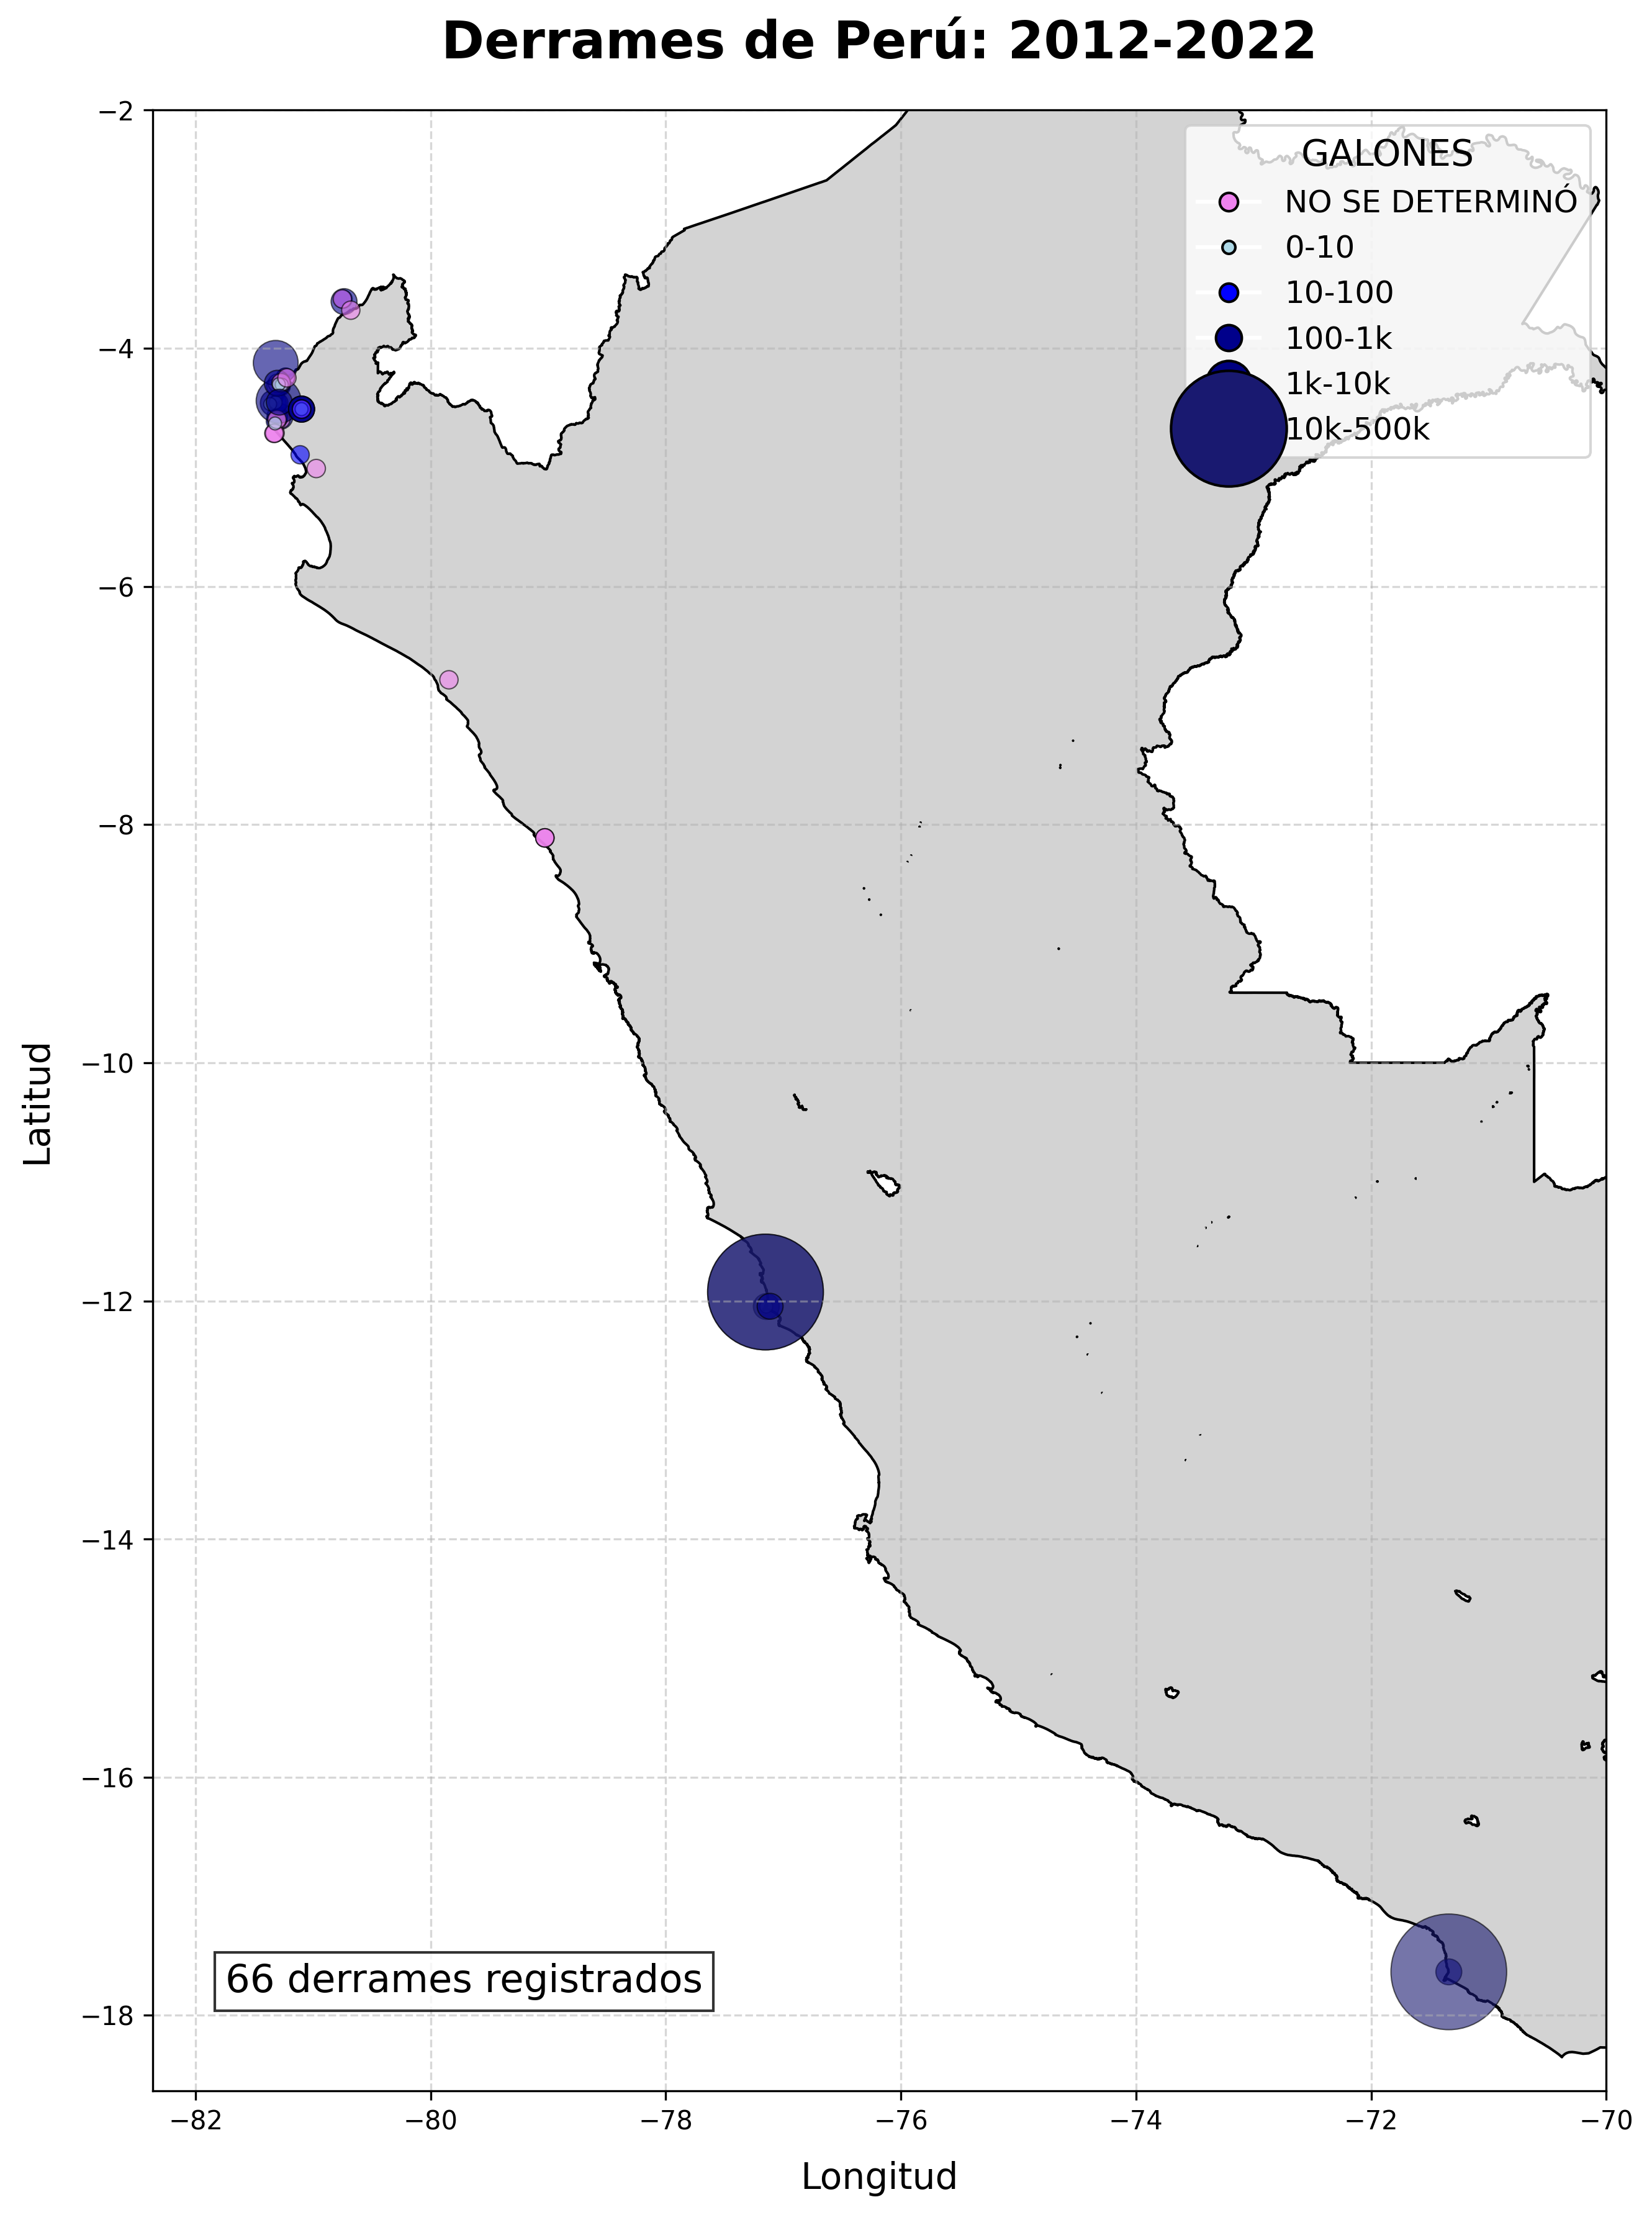
\includegraphics[width=1\textwidth]{figures/oil_spills_map_peru.png}
    \caption{Spatial distribution and volume classification of 66 oil spills recorded along the Peruvian coast from 2012 to 2022.}
    \label{fig:peru_spills_map}
\end{figure}

A total of 40 Sentinel-1 SAR images were ultimately selected from this set of events based on three criteria: (1) visual observability of the oil slick in the SAR image, (2) temporal proximity to the reported spill date (within 3–20 days, following \cite{mogollonREPSOLOilSpill2023}), and (3) availability and quality of satellite acquisition. These images span the period from 2014 to 2025 and were acquired from the Copernicus Sentinel-1 archive.

From each selected image, non-overlapping patches of 512$\times$512 pixels were manually extracted around areas containing oil and other semantically relevant features (e.g., vessels, land, open sea). This patch-based strategy was adopted to mitigate class imbalance by avoiding excessive background pixels. A total of 2,132 patches were obtained, with 1,820 (approx. 85\%) used for training and 312 (15\%) for testing. The train-test split was applied at the image level to ensure semantic independence between sets.

Table~\ref{tab:peruvian_selection} summarizes the 40 Sentinel-1 SAR scenes selected for the Peruvian coastal dataset, sorted chronologically by spill date. Each entry corresponds to a confirmed spill case, including its coordinates, SAR acquisition date, and delay in days (\textit{Δ Days}) between the incident and image capture.

The number of extracted patches per image varies depending on the spill extent and visual clarity, aiming to maximize coverage of oil-related features while limiting background noise. This structured selection and labeling process ensures class balance, spatial diversity, and robustness in model training and evaluation.


\vspace{1em}
Each row in the table represents a real-world spill case. The \textit{Δ Days} column highlights the critical time window between the spill incident and the satellite acquisition. The number of extracted patches per image reflects the spatial extent of relevant content while prioritizing oil spill regions and avoiding class imbalance.

\subsection{Preprocessing}
All images are radiometrically calibrated to $\sigma^0$, 
received speckle noise reduction (3$\times$3 median), and normalized to 10 m/pixel. 
Peruvian scenes also undergo terrain flattening and simple incidence-angle normalization. 
We retain only IW swath, VV polarization. Details on implementation are provided in Appendix~A.
\subsubsection{Domain Differences}
Despite relying on the same SAR sensor (Sentinel-1 GRD, VV polarization), the Mediterranean and Peruvian datasets exhibit distinct environmental and acquisition conditions that pose challenges for generalization and motivate the use of domain adaptation techniques (see \ref{tab:domain_differences}.

These domain shifts affect the visual appearance of oil slicks and background patterns in SAR images, which can degrade the performance of models trained in one region when applied to another. Therefore, domain adaptation becomes essential to improve generalization to new environmental conditions.

\begin{table}[ht]
\centering
\caption{Key differences between the Mediterranean and Peruvian SAR datasets.}
\begin{tabular}{|p{3.5cm}|p{5.2cm}|p{5.2cm}|}
\hline
\textbf{Aspect} & \textbf{Mediterranean Dataset} & \textbf{Peruvian Dataset} \\
\hline
Sea conditions & Calmer, semi-enclosed seas (e.g., Aegean) with smaller slicks & Rougher open-sea conditions; larger and more irregular slicks \\
\hline
Oceanographic forcing & Moderate seasonal winds and currents & Strong Humboldt Current, frequent upwelling zones \\
\hline
SAR backscatter texture & Smooth background, high contrast between slick and sea & Textured background, increased risk of misclassification \\
\hline
Acquisition geometry & Primarily descending orbits; narrow range of incidence angles & Mixed orbits; wider variation in incidence angles and surface response \\
\hline
Ground truth quality & Detailed EMSA CleanSeaNet reports and segmentation masks & Sparse ground truth from OEFA/OSINERGMIN; manual annotations required \\
\hline
\end{tabular}
\label{tab:domain_differences}
\end{table}
\clearpage

\subsection{Deep Learning Segmentation Models} 
We benchmark four representative families under a unified training setup to provide a robust baseline for oil-spill segmentation.

\paragraph{ResNet-UNet (R34).}
A standard UNet decoder with skip connections on top of a ResNet-34 encoder (ImageNet pretraining). This serves as our canonical encoder–decoder baseline~\cite{ronnebergerUNetConvolutionalNetworks2015a,heDeepResidualLearning2015}.

\paragraph{ResNet-UNet + ASPP (R34+ASPP).}
A practical variant that inserts an Atrous Spatial Pyramid Pooling (ASPP) block at the bottleneck to capture multi-scale context with minimal overhead; we treat this as a baseline variant rather than a novel architecture~\cite{chenDeepLabSemanticImage2017}.

\paragraph{DeepLabV3\textplus{} (R34).}
A lightweight head that aggregates multi-scale features via ASPP and uses a single low-level skip to refine boundaries, replacing a heavy UNet-style decoder~\cite{chenDeepLabSemanticImage2017}.

\paragraph{TransUNet.}
A CNN encoder feeding a ViT core to model long-range dependencies, followed by a UNet-style decoder~\cite{chenTransUNetTransformersMake2021}.

\paragraph{EfficientNetV2-M + DeepLabV3\textplus{}.}
An EfficientNetV2-M encoder paired with a DeepLabV3\textplus{} head to probe accuracy–efficiency trade-offs~\cite{efsongEfficientMarineOil2018,chenDeepLabSemanticImage2017}.

\paragraph{Fairness controls.}
All backbones use the same input size ($512{\times}512$), class set, loss (CE{+}Dice), class weights, data augmentation, optimizer/schedule, epochs, and seeds; only the backbone/head differ. We report mean$\pm$std over three seeds. Implementation details and hyperparameters are in Appendix~A.


\subsection{Synthetic Data Generation}
We synthesize SAR-like patches from 5-class semantic masks using a SPADE generator with
Instance-Adaptive De-normalization (INADE) \cite{park2019spade, tan2021inade}. SPADE modulates
normalization parameters spatially from the input mask, preventing the semantic information from
being washed out by vanilla normalization \cite{park2019spade}. INADE further samples instance-level
modulation to increase diversity across objects of the same class \cite{tan2021inade}.
The discriminator uses spectral normalization and a hinge loss to stabilize training \cite{miyato2018spectral},
and we adopt Adam with TTUR-style learning rates \cite{heusel2017ttur}.
We trained for 60 epochs on $512{\times}512$ crops with $D{:}G=1{:}1$, $\lambda_\text{feat}{=}10$,
$\lambda_\text{VGG}{=}10$, and $\text{lr}{=}5{\times}10^{-5}$.
While diffusion models can surpass GANs in sample quality, their iterative sampling cost renders them
impractical for large-batch augmentation in our setting \cite{dhariwal2021diffusion, yang2022diffsurvey}.



\subsection{MORP: Morphological Region Perturbation}
\label{sec:morp}

We propose \textbf{MORP-Synth}, a two-stage pipeline that augments scarce SAR oil-spill training data by
(1) perturbing object \emph{shape} directly in label space via our Morphological Region Perturbation (\textbf{MORP}), and
(2) rendering SAR-like appearance from the edited masks using an off-the-shelf conditional generator (SPADE with INADE).
Our novelty lies in Stage~A; Stage~B is an applied component selected for efficiency and controllability.


\subsection{Stage A: MORP—Morphological Region Perturbation}
\label{sec:morp-main}
MORP edits spill shapes in the label domain while preserving surrounding context. Given a $K$-class mask
($K{=}5$: sea, oil, look-alike, ship, land), we (i) select target connected components ($\mathcal{C}{=}\{\text{oil},\text{look-alike}\}$),
(ii) apply a single rigid move per selected region (erase$\to$rotate$\to$translate$\to$paste with collision rejection),
(iii) detect boundary \emph{apices} via smoothed curvature peaks, and (iv) perform localized stochastic edits
(bulge or wedge) along outward normals. The result is an augmented mask $\mathcal{L}^\star$ with realistic
lobes/notches and plausible displacements (Algorithm~\ref{alg:morp}) that can be rendered into SAR-like geometry objects appearance.

\paragraph{Defaults (replicable).}
Unless stated otherwise, we use: $\theta \sim \mathcal{U}[-\pi,\pi)$, translation radius $r\!\sim\!\mathcal{U}[0,120]$\,px with random direction,
$m{=}6$ apices/region, expansion prob.\ $p_{\mathrm{exp}}{=}0.6$, fan half-angle $\alpha{=}60^\circ$,
$r_{\max}{=}50$\,px, $n_{\mathrm{rays}}{=}120$, Savitzky–Golay smoothing ($w{=}9$, $p{=}3$),
peak-prominence at the 85th percentile of positive curvature with $\ge4$\,px spacing.
Random seeds are fixed for determinism in ablations.




\begin{algorithm}[H]
\caption{MORP (minimal pipeline)}
\label{alg:morp}
\begin{algorithmic}[1]
\Require Label map $\mathcal{L}\in\{0,\dots,4\}^{H\times W}$; target classes $\mathcal{C}=\{1,2\}$
\Require Transform params: angle range $[-\pi,\pi)$, max shift $R$
\Require Apex params: $m$ apices, $p_{\mathrm{exp}}$, fan half-angle $\alpha$, rays $n_{\mathrm{rays}}$, max radius $r_{\max}$
\Ensure Augmented labels $\mathcal{L}^\star$
\State $\mathcal{L}^\star \gets \mathcal{L}$
\State $\mathcal{R} \gets \bigcup_{c\in\mathcal{C}}\mathrm{ConnComp}(\mathbb{1}[\mathcal{L}{=}c])$ \Comment{connected components of oil/look-alike}
\ForAll{$R \in \mathrm{Select}(\mathcal{R})$} \Comment{e.g., $4$–$8$ regions/image, stratified by class}
  \State $c \gets \mathrm{Class}(R)$
  \State \textit{// Stage 1: rotate \& place}
  \State sample $\theta$ and $(\Delta x,\Delta y)$ with $\|\!(\Delta x,\Delta y)\!\|\le R$
  \State $R_{\mathrm{rot}} \gets \mathrm{RotateNoCrop}(R,\theta)$
  \State $\mathcal{L}^\star \gets \mathrm{EraseRegion}(\mathcal{L}^\star,R)$
  \If{$\mathrm{TryPaste}(\mathcal{L}^\star,R_{\mathrm{rot}},\Delta x,\Delta y, \text{allowed}=\{0,3\})$}
    \State $R' \gets \mathrm{ExtractRegion}(\mathcal{L}^\star,c,\text{near paste})$
    \State \textit{// Stage 2: apices on the new boundary}
    \State $A \gets \mathrm{FindApicesViaCurvature}(R',\, w{=}9,\, p{=}3,\, \text{prominence}=85{\small th}\%)$
    \State choose $m$ points $A_m \subseteq A$ (enforce min spacing)
    \State \textit{// Stage 3: multi-apex stochastic edits}
    \ForAll{$a \in A_m$}
      \State $B,S \gets \mathrm{ApexEdit}(R', a, p_{\mathrm{exp}}, \alpha, n_{\mathrm{rays}}, r_{\max})$
      \State \textbf{if} $B\!\neq\!\emptyset$ \textbf{ then } $\mathcal{L}^\star[B]\gets c$ \Comment{union (bulge)}
      \State \textbf{if} $S\!\neq\!\emptyset$ \textbf{ then } $\mathcal{L}^\star[S]\gets 0$ \Comment{difference (shrink)}
    \EndFor
  \Else
    \State \textbf{continue} \Comment{reject placement, keep map unchanged}
  \Fi
\EndFor
\State \Return $\mathcal{L}^\star$
\end{algorithmic}
\end{algorithm}

\begin{algorithm}[H]
\caption{FindApicesViaCurvature (contour peaks)}
\label{alg:apices}
\begin{algorithmic}[1]
\Require Region mask $R'$, smoothing window $w$, polyorder $p$, peak prominence quantile $q{=}0.85$
\Ensure Set of apex coordinates $A$
\State $P \gets \mathrm{OuterContour}(R')$ \Comment{ordered $(x_t,y_t)$, $t{=}1..N$}
\State $(\tilde{x},\tilde{y}) \gets \mathrm{SavitzkyGolay}(x,y; w,p,\text{mode=wrap})$
\State compute discrete curvature $\kappa_t$ from $(\tilde{x}_t,\tilde{y}_t)$
\State $\kappa^{+}_t \gets \max(0,\kappa_t)$; threshold $\tau \gets \mathrm{Quantile}(\{\kappa^{+}_t\},q)$
\State $\text{peaks} \gets \mathrm{FindPeaks}(\kappa^{+},\text{prominence}>\tau,\text{distance}\ge4)$
\State \Return $A \gets \{(\tilde{x}_t,\tilde{y}_t)\,:\, t\in\text{peaks}\}$
\end{algorithmic}
\end{algorithm}

\begin{algorithm}[H]
\caption{ApexEdit (expand or shrink at a point)}
\label{alg:apexedit}
\begin{algorithmic}[1]
\Require Region mask $R'$, apex $a$, prob.\ $p_{\mathrm{exp}}$, fan half-angle $\alpha$, ray count $n_{\mathrm{rays}}$, max radius $r_{\max}$
\Ensure Add-mask $B$ (bulge), remove-mask $S$ (wedge)
\State $B,S \gets \emptyset,\emptyset$
\State $\vec{n} \gets \mathrm{NormalAt}(R',a)$ \Comment{e.g., gradient of distance transform}
\State $z \sim \mathrm{Bernoulli}(p_{\mathrm{exp}})$
\If{$z{=}1$} \Comment{expand}
  \State $B \gets \mathrm{RadialFanPolygon}(a,\vec{n},\alpha,n_{\mathrm{rays}},r_{\max},\text{smooth/close})$
\Else \Comment{shrink}
  \State $S \gets \mathrm{RadialFanPolygon}(a,-\vec{n},\alpha,n_{\mathrm{rays}},r_{\max},\text{smooth/close}) \cap R'$
\EndIf
\State \Return $B,S$
\end{algorithmic}
\end{algorithm}

\vspace{-0.25em}
\paragraph{Symbols (quick reference).}
\begin{center}
\begin{tabular}{@{}ll@{}}
\toprule
Symbol & Meaning \\
\midrule
$\mathcal{L}$ & input labels (classes: sea, oil, look-alike, ship, land) \\
$\mathcal{C}$ & target classes $\{1,2\}$ (\emph{oil}, \emph{look-alike}) \\
$R, R', R_{\mathrm{rot}}$ & original region, pasted region, rotated region \\
$A, A_m$ & all apices, chosen subset for edits \\
$\alpha, n_{\mathrm{rays}}, r_{\max}$ & fan half-angle, ray count, max radial extent \\
$B, S$ & add-mask (bulge), remove-mask (shrink) \\
\bottomrule
\end{tabular}
\end{center}


\begin{figure}[htbp]
  \centering
  % Center the entire table
  \makebox[\textwidth][c]{
  \renewcommand{\arraystretch}{1.0}
  \setlength{\tabcolsep}{3pt}
  \begin{tabular}{c}
    %── Header text ───────────────────────────────────────────────
    \textbf{\scriptsize (a) Original \quad (b) Rotate \& Place + Apices Selection 
    \quad (c) Curvature Edits (+ / –) 
    \quad (d) Final Augmented Image} \\[0.3em]
    %── Row 1 ─────────────────────────────────────────────────────
    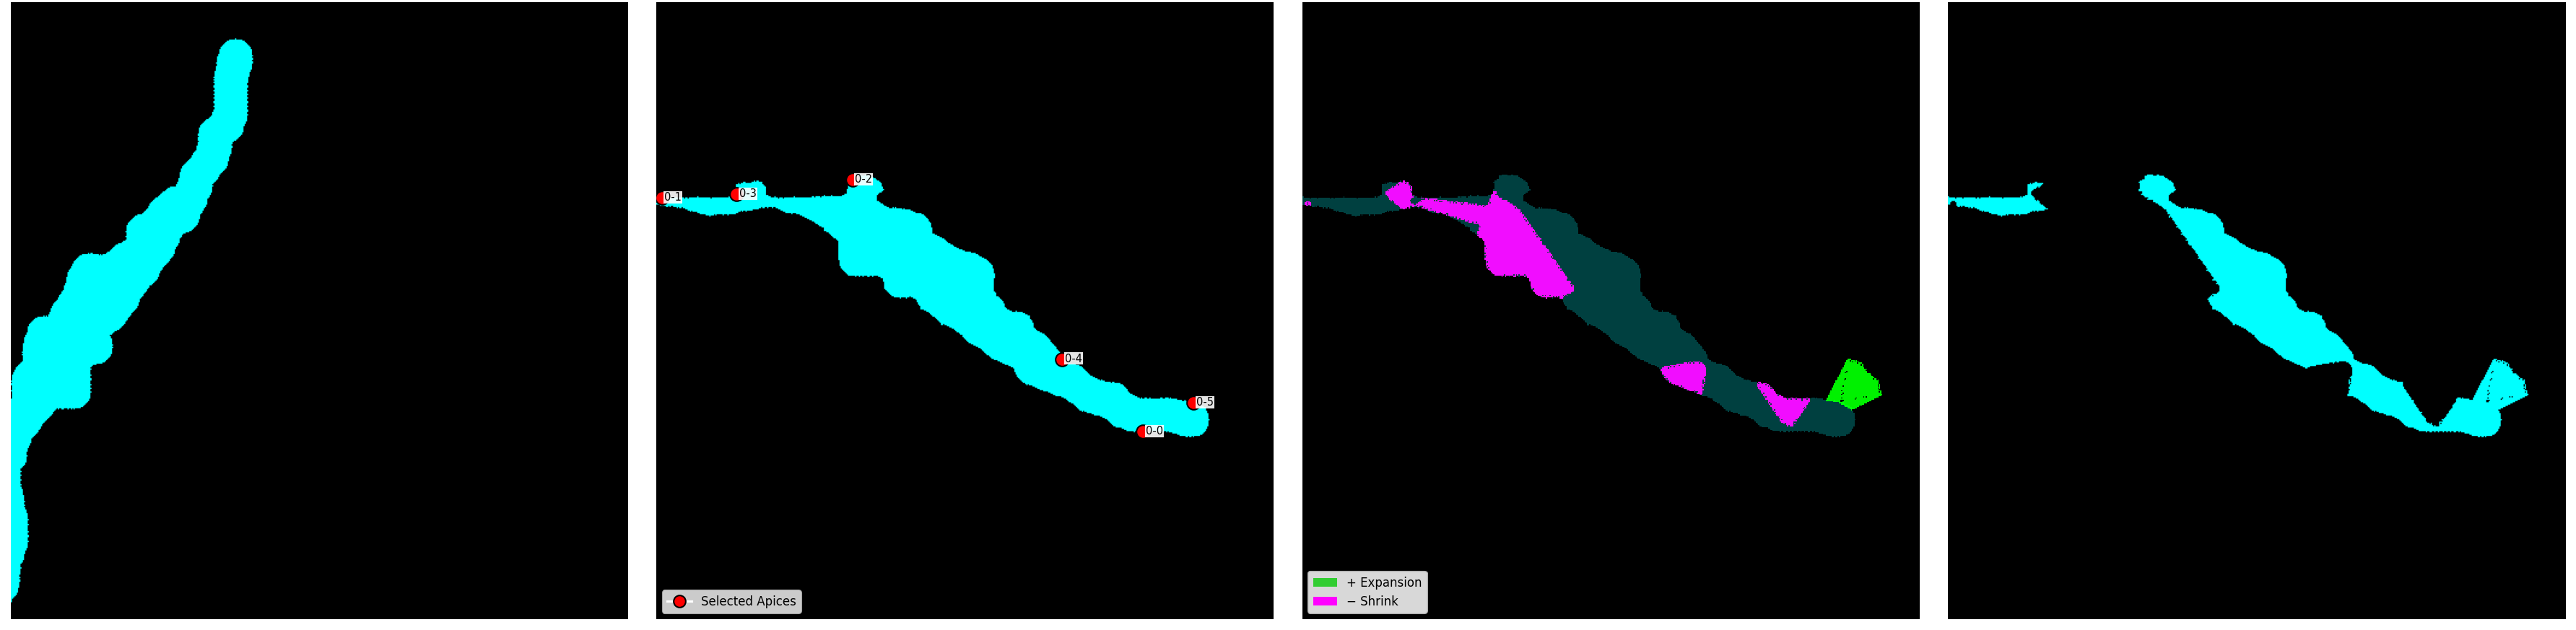
\includegraphics[width=0.93\textwidth]{figures/images_morp/img_6__GLOBAL_summary_rgb.png} \\[0.6em]
    %── Row 2 ─────────────────────────────────────────────────────
    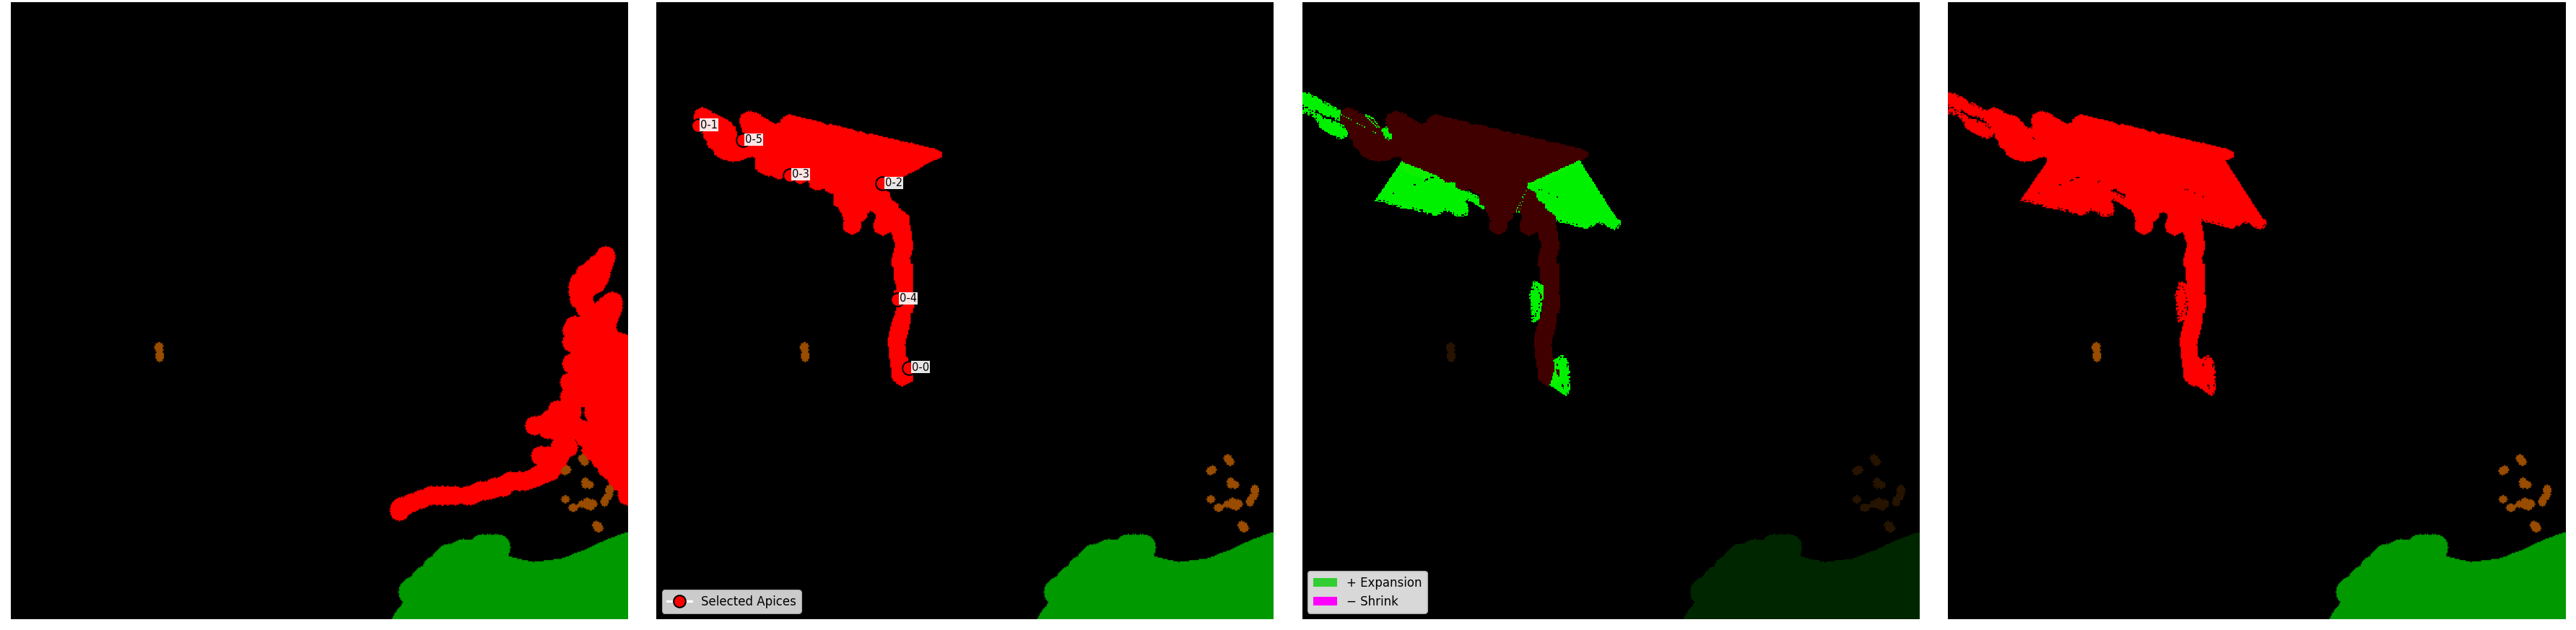
\includegraphics[width=0.93\textwidth]{figures/images_morp/img_7__GLOBAL_summary_rgb.png} \\
  \end{tabular}
  }

  \caption{Illustration of the MORP augmentation workflow for two representative spill regions.
  Each row shows the complete four-stage process within a single image:
  (a) original mask before transformation; 
  (b) rotated/translated region with detected apices; 
  (c) curvature-based local edits showing expansions (magenta) and shrinkages (green); 
  (d) final augmented mask after shape perturbation.
  Additional examples are provided in Appendix~A.}
  \label{fig:morp_workflow}
\end{figure}



\subsection{Stage B: Mask-to-SAR Synthesis (cGAN-INADE)}
\label{sec:gen}
We condition an off-the-shelf SPADE generator~\cite{park2019spade} augmented with
Instance-Adaptive De-normalization (INADE)~\cite{tan2021inade} on the edited masks.
SPADE sets per-pixel affine normalization from the semantic mask to preserve structure,
while INADE samples instance-level modulation to diversify shapes of the same class.


\begin{figure}[htbp]
  \centering
  \makebox[\textwidth][c]{
  \renewcommand{\arraystretch}{1.0}
  \setlength{\tabcolsep}{3pt}
  \begin{tabular}{cccc}
    \textbf{\scriptsize (a) Real SAR} & 
    \textbf{\scriptsize (b) Real Mask} & 
    \textbf{\scriptsize (c) Synthesized Mask (MORP) } & 
    \textbf{\scriptsize (d) Synthesized SAR (INADE)} \\[0.4em]
    %─── Row 1 ───────────────────────────────────────────────
    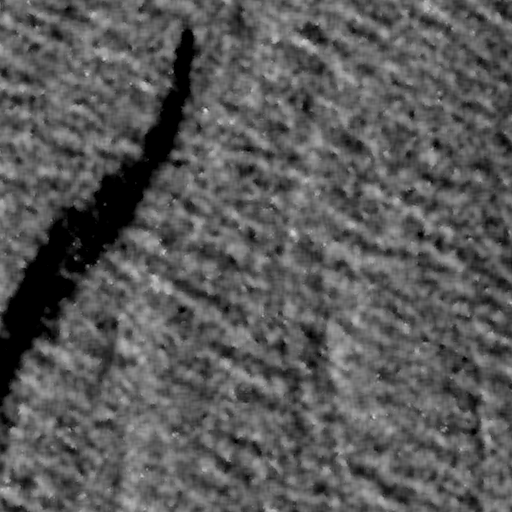
\includegraphics[width=0.22\textwidth]{figures/images_morp/inade_trans_pairs/7_1_2015-03-16_S1_GRD_VV_patch_21-1.png} &
    
\includegraphics[width=0.22\textwidth]{figures/images_morp/inade_trans_pairs/7_1_2015-03-16_S1_GRD_VV_mask1d_21_rgb.png} &
    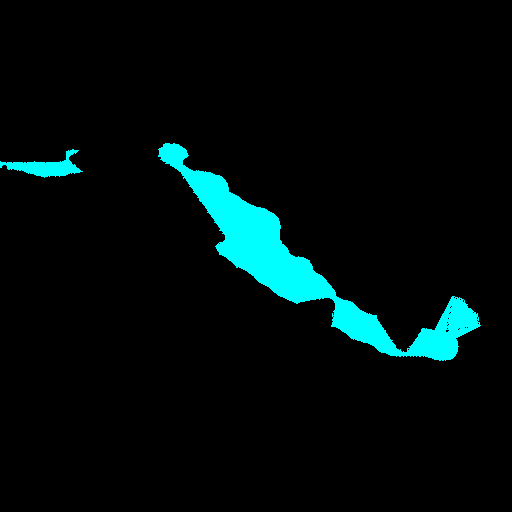
\includegraphics[width=0.22\textwidth]{figures/images_morp/inade_trans_pairs/aug_lookalike_rgb_7_1_2015-03-16_S1_GRD_VV_mask1d_21.png} &
    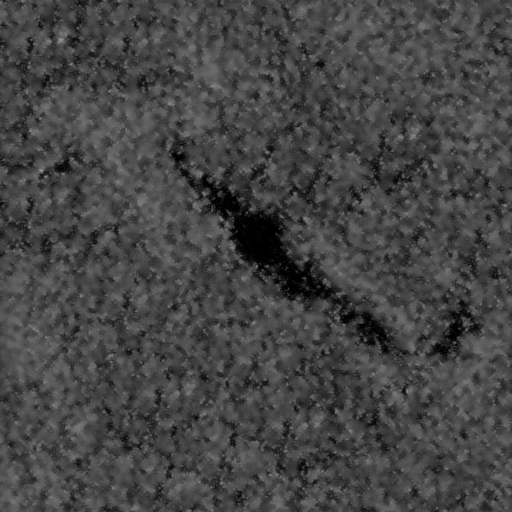
\includegraphics[width=0.22\textwidth]{figures/images_morp/inade_trans_pairs/aug_lookalike_label_7_1_2015-03-16_S1_GRD_VV_mask1d_21.png} \\[0.6em]
    %─── Row 2 ───────────────────────────────────────────────
    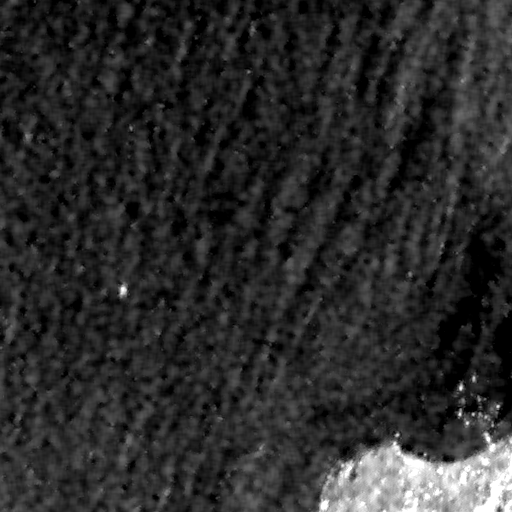
\includegraphics[width=0.22\textwidth]{figures/images_morp/inade_trans_pairs/95_1_2017-07-18_S1_GRD_VVVH_patch_0-1.png} &
    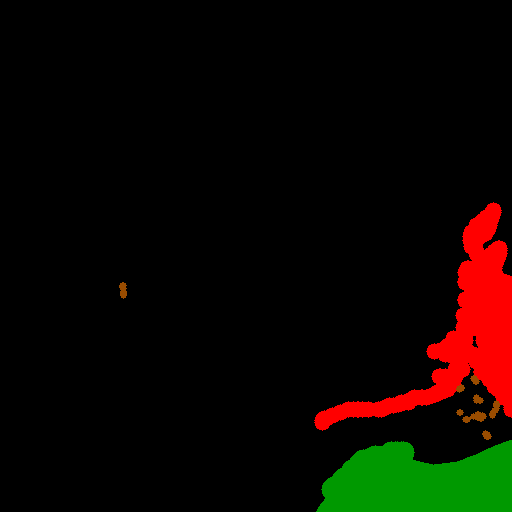
\includegraphics[width=0.22\textwidth]{figures/images_morp/inade_trans_pairs/95_1_2017-07-18_S1_GRD_VVVH_mask1d_0_rgb.png} &
    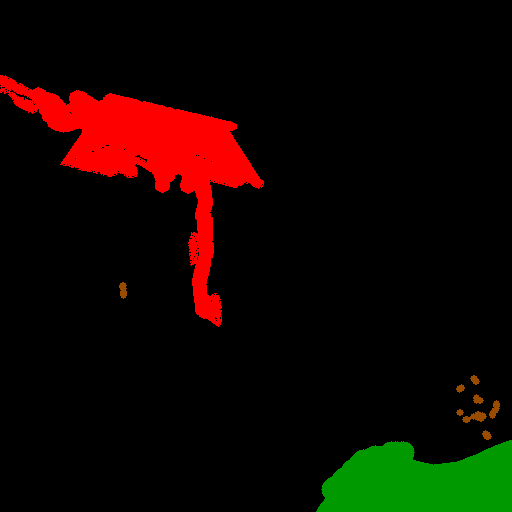
\includegraphics[width=0.22\textwidth]{figures/images_morp/inade_trans_pairs/aug_lookalike_rgb_95_1_2017-07-18_S1_GRD_VVVH_mask1d_0.png} &
    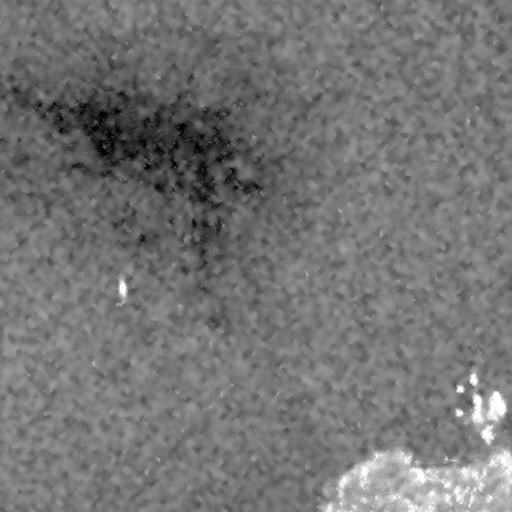
\includegraphics[width=0.22\textwidth]{figures/images_morp/inade_trans_pairs/aug_lookalike_label_95_1_2017-07-18_S1_GRD_VVVH_mask1d_0.png} \\
  \end{tabular}
  }

  \caption{Comparison of real and synthesized samples in the Mask-to-SAR generation stage using SPADE with Instance-Adaptive De-Normalization (INADE). 
  Columns show: (a) real Sentinel-1 SAR patches; (b) corresponding ground-truth masks; 
  (c) synthetic SAR images generated by SPADE+INADE conditioned on MORP-augmented masks; 
  (d) synthesized masks produced by MORP. The generated patches preserve object geometry while introducing realistic backscatter variation.}
  \label{fig:inade_synth_pairs}
\end{figure}







\paragraph{Training details.}
Unless stated, we train for 60 epochs on $512{\times}512$ crops using Adam with TTUR-style learning rates
($D{:}G=1{:}1$, $\lambda_\text{feat}{=}10$, $\lambda_\text{VGG}{=}10$, $\text{lr}{=}5{\times}10^{-5}$),
a spectrally normalized discriminator with hinge loss~\cite{miyato2018spectral,heusel2017ttur}.
While diffusion models can exceed GANs in sample quality, their iterative sampling cost renders them impractical
for large-batch augmentation in our setting~\cite{dhariwal2021diffusion,yang2022diffsurvey}.

\subsection{Putting it together}
Given a real mask $\mathcal{L}$, MORP produces $\mathcal{L}^\star$ (Stage~A), which conditions the generator
to yield a synthetic SAR patch $x^\star$ (Stage~B). We pair $\{x^\star,\mathcal{L}^\star\}$ with real
$\{x,\mathcal{L}\}$ to train a segmentation model. Section~\ref{sec:exp} quantifies gains from
MORP (shape edits) vs.\ synthesis (appearance) via controlled ablations.







\subsubsection{Sampling Strategy}

\subsubsection{Training Details}
\label{sec:training}

All models are first trained from scratch on the Krestinin Mediterranean dataset, consisting of 4 962 non-overlapping 512 × 512 tiles, with 569 held out for test.  We then fine-tune on the Peruvian set (3640 train , 312 test).  Half of the patches extracted contains some portion of oil spill or look alike and the other half do not, this is because we want to make sure to reduce the false positive rate of imbalanced presence wise images \cite{deandradeImprovedSegmentationExtreme2024}. This train & test split is done by spill event (41 cases) (See Table~\ref{tab:peruvian_selection})  

We optimize a composite loss   
\[
\mathcal{L} \;=\; \mathcal{L}_{\mathrm{WCE}} \;+\; \mathcal{L}_{\mathrm{Dice}},
\]  
where the weighted cross-entropy weight for class \(c\) is set proportional to the geometric mean of its pixel frequency over all training images.

Training uses the Adam optimizer with initial learning rate \(\eta=1\times10^{-4}\), weight decay \(10^{-4}\), and batch size 32.  We pretrain for 60 epochs on the Krestinin data (4 962 tiles), applying on-the-fly augmentations via Albumentations: random horizontal and vertical flips, Gaussian noise, CoarseDropout (up to eight holes of size up to 32×32).


After pretraining converges, we fine-tune both the Freeze-Backbone and Full Fine-Tuning protocols for 20 additional epochs each, increasing the head learning rate to \(2\times10^{-4}\) while keeping encoder rates unchanged.  Checkpointing, ReduceLROnPlateau (factor 0.3, patience 5), and early stopping (patience 7) ensure stable convergence.  


\subsubsection{Evaluation Metrics}
\label{sec:evaluation}

\paragraph{Mean Intersection-over-Union (mIoU)}  
We evaluate segmentation performance using the mean Intersection-over-Union (mIoU) over all \(C=5\) semantic classes. For each class \(c \in \{0,\dots,4\}\), the IoU is defined as:
\[
\mathrm{IoU}_c = \frac{\mathrm{TP}_c}{\mathrm{TP}_c + \mathrm{FP}_c + \mathrm{FN}_c},
\]
where \(\mathrm{TP}_c\), \(\mathrm{FP}_c\), and \(\mathrm{FN}_c\) are the number of true positives, false positives, and false negatives for class \(c\), respectively. 

\paragraph{False‐Positive Rate on Pure‐Sea Scenes}  
To quantify robustness against false detections, we compute the false-positive rate (FPR) on a curated set of “pure-sea” validation tiles—patches that contain no oil or look-alike pixels. Let \(\hat{y}_{i,j}\) be the predicted class label at pixel \((i,j)\), where class 0 corresponds to background (sea surface). Then, the FPR is:
\[
\mathrm{FPR} = \frac{1}{HW} \sum_{i,j} \mathbf{1}\left\{ \hat{y}_{i,j} \neq 0 \right\},
\]
i.e., the proportion of non-background pixels predicted in a patch that should be entirely clean water. This metric is critical to assess over-segmentation and operational reliability in real-world scenarios where oil spills are rare.
\subsection{Experimental Design and Training Strategy}


\section{Results}

\subsection{Quantitative Evaluation}


\subsubsection{Baseline (Source-only)}

\begin{figure}[H]
\centering

\begin{subfigure}[b]{0.48\textwidth}
  \centering
  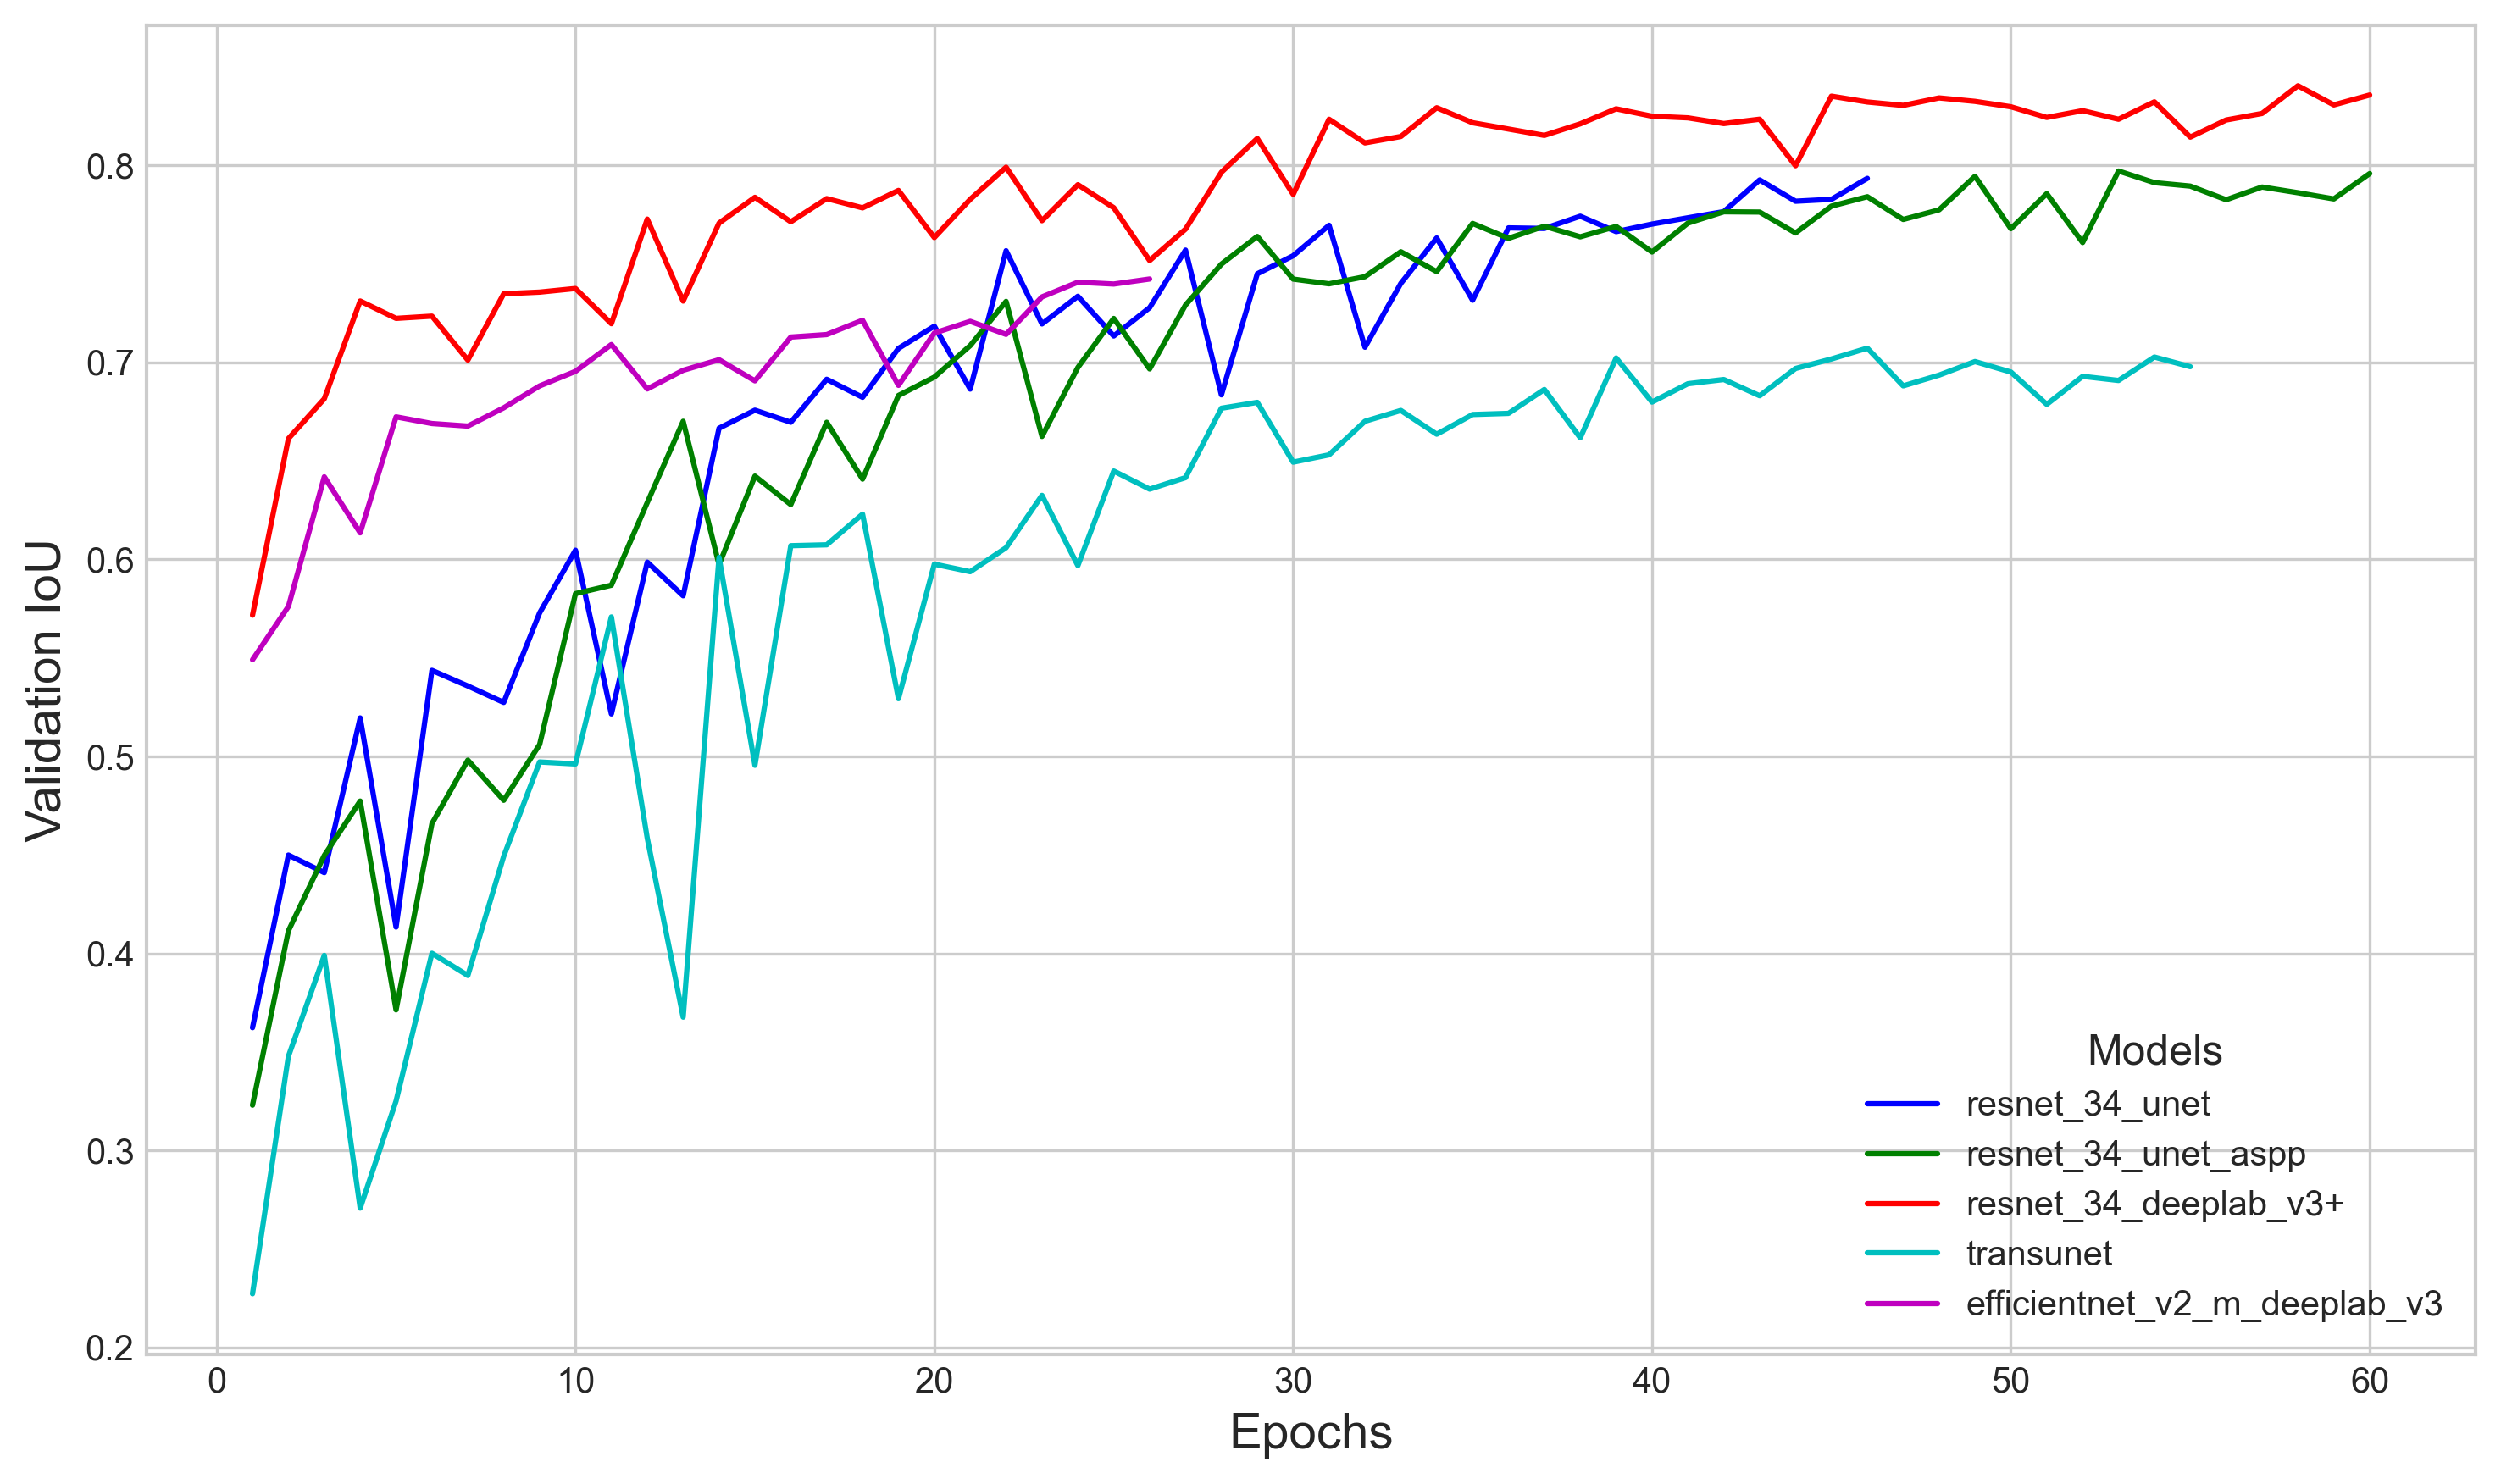
\includegraphics[width=\textwidth]{figures/valid_iou_vs_epochs_academic.png}
  \caption{Validation IoU vs.\ epochs}
  \label{fig:iou_epochs}
\end{subfigure}
\hfill
\begin{subfigure}[b]{0.48\textwidth}
  \centering
  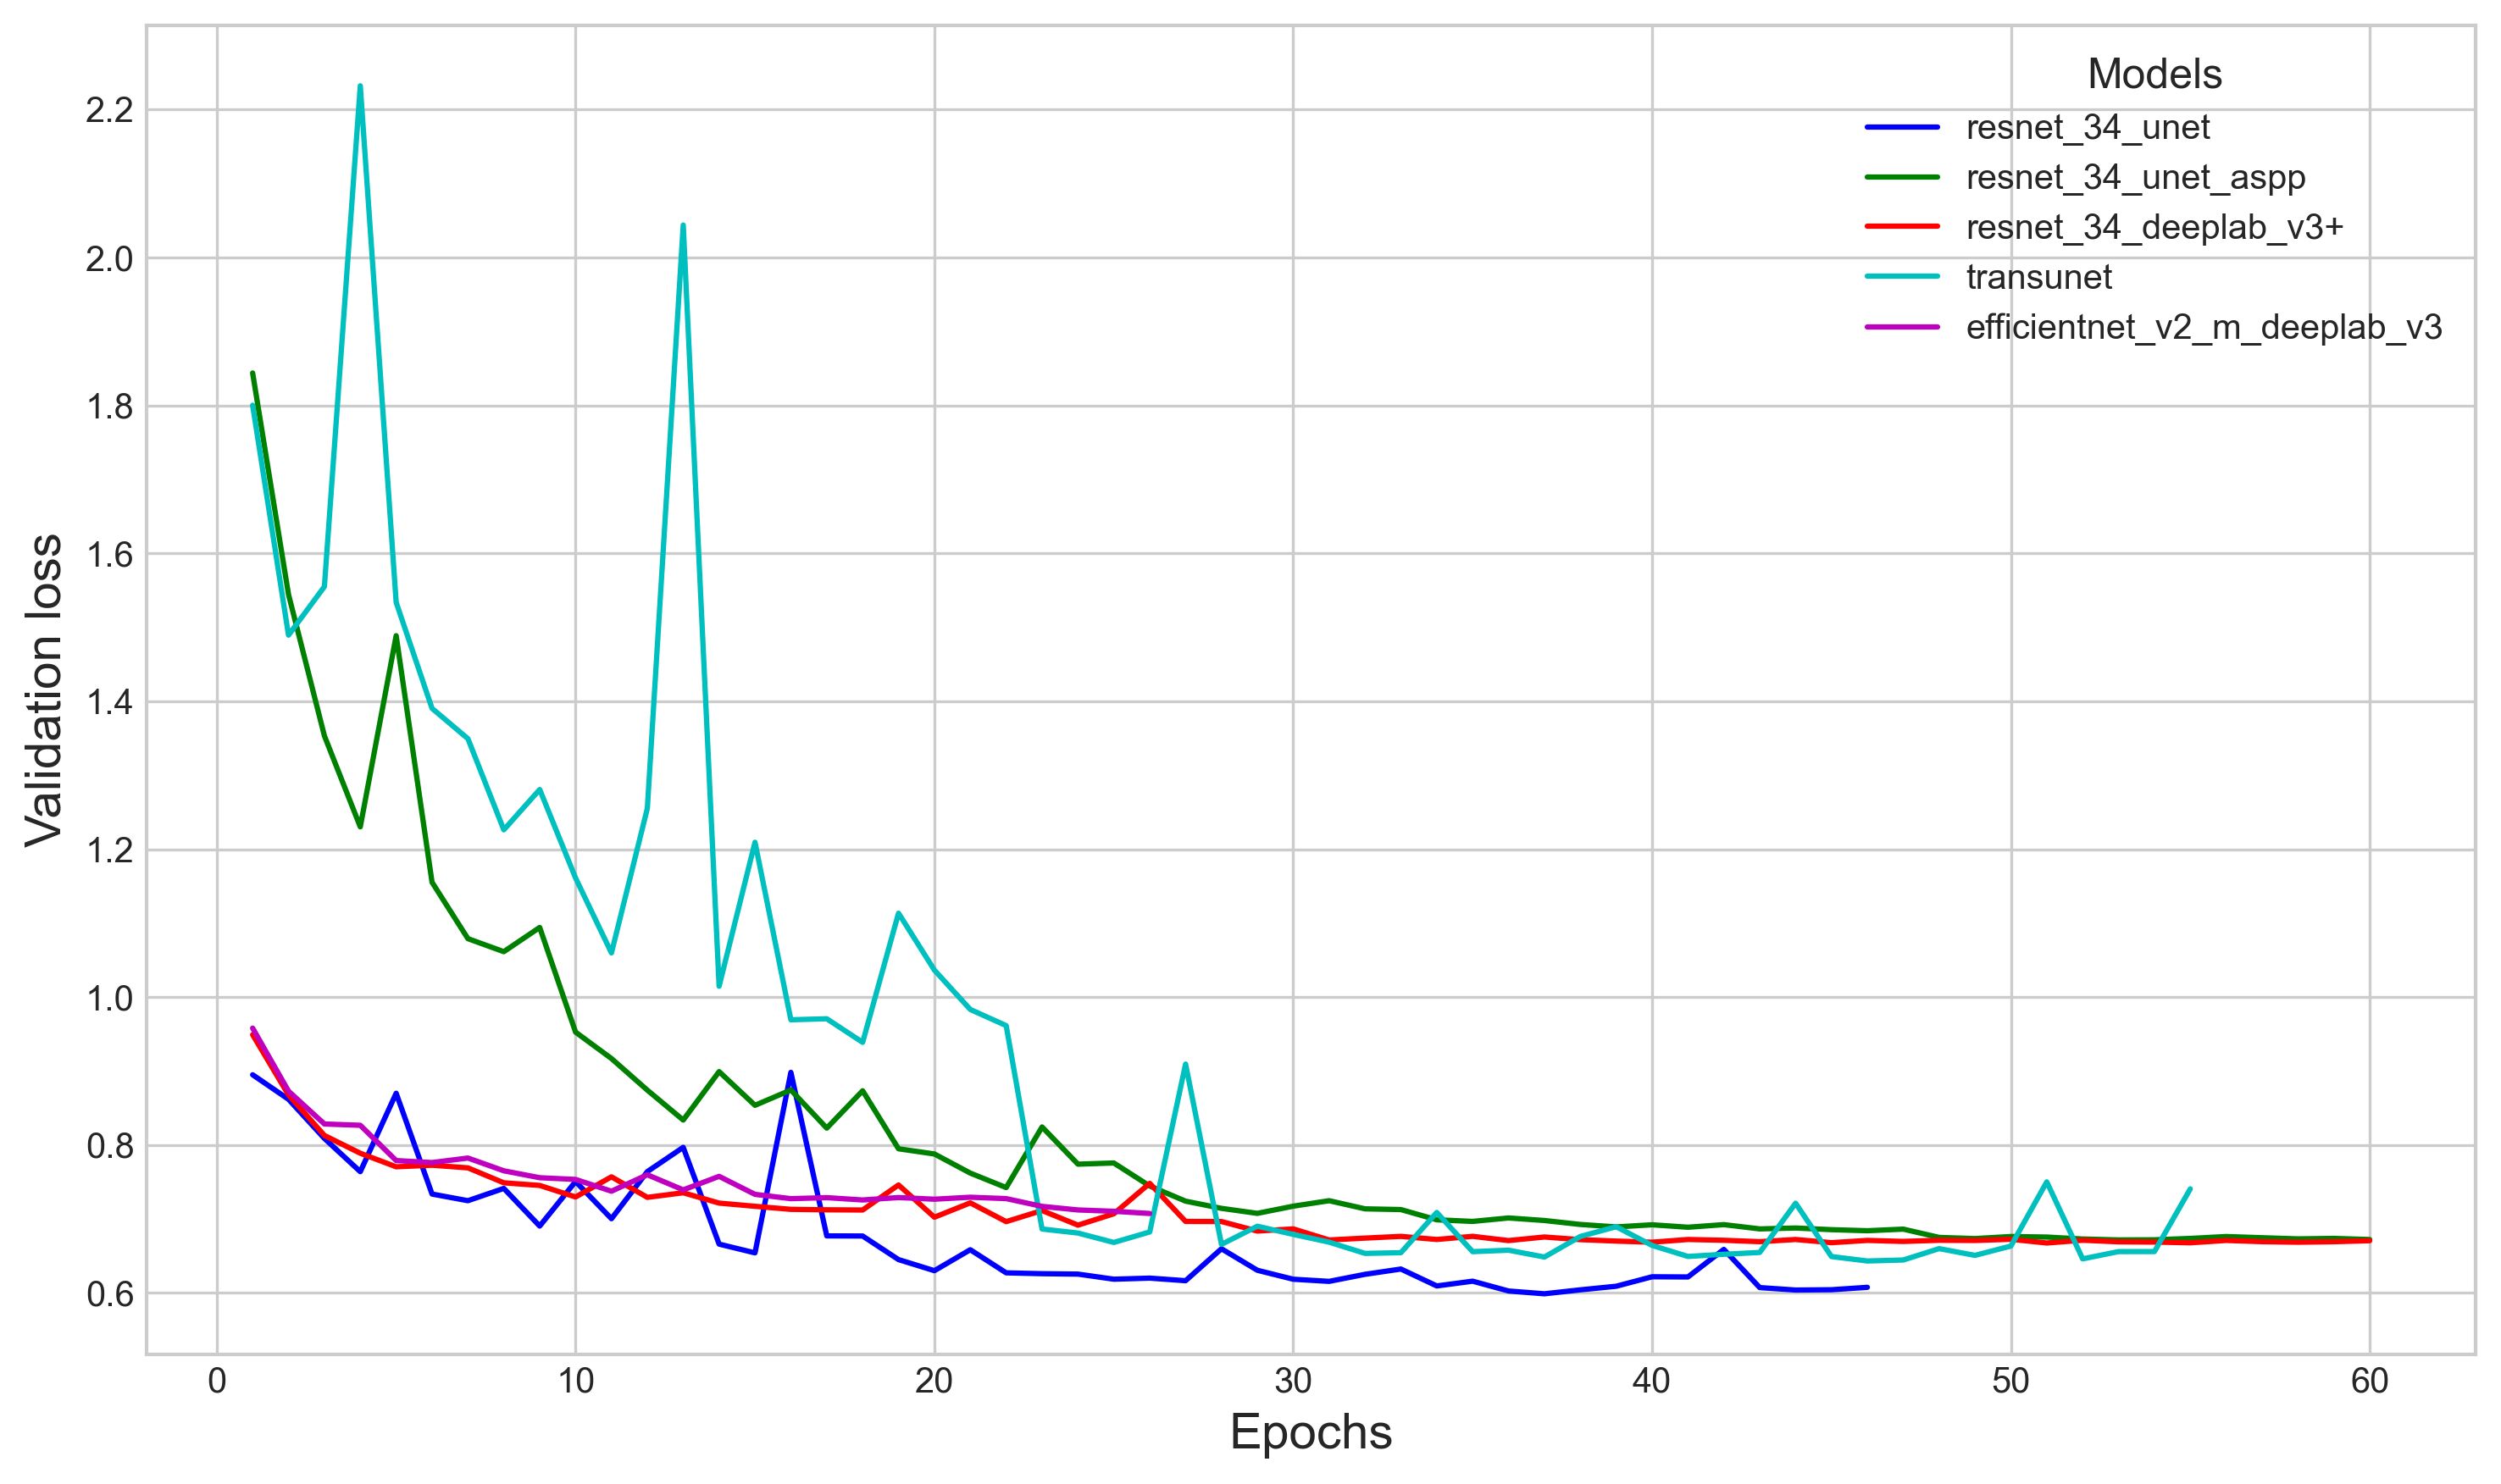
\includegraphics[width=\textwidth]{figures/valid_loss_vs_epochs_academic.png}
  \caption{Validation loss vs.\ epochs}
  \label{fig:loss_epochs}
\end{subfigure}

\caption{Training curves on the Krestinin source domain: (a) validation mean IoU over 60 epochs; (b) validation loss over 60 epochs.}
\label{fig:training_krestinin}
\end{figure}
Prior to domain adaptation, all five architectures (ResNet-34 UNet, ResNet-34 UNet+ASPP, ResNet-34 DeepLabV3\texttt{+}, TransUNet, and EfficientNetV2-M + DeepLabV3) were trained for 60 epochs on the Krestinin dataset (4 962 non-overlapping 512×512 tiles, with 569 held out for validation). As shown in Figure~\ref{fig:iou_epochs}, validation IoU rises sharply in the first 20 epochs and then gradually decreases between 0.75 and 0.85, with DeepLabV3\texttt{+} converging earliest and to the highest IoU. Figure~\ref{fig:loss_epochs} confirms a smooth decrease in validation loss, with no signs of premature overfitting. These preliminary results demonstrate that all encoders and decoders learned robust source-domain representations before the evaluation in Table~\ref{tab:krestinin_test}.


Table~\ref{tab:krestinin_test} summarizes the performance of all evaluated architectures on the unseen Krestinin test set of 569 tiles (\(512\times512\)). Among all baselines, the \textit{ResNet-34 DeepLabV3\texttt{+}} achieved the highest mean IoU (67.82\%), followed closely by the \textit{ResNet-34 UNet+ASPP} (66.05\%) and the plain \textit{UNet} (65.82\%). These results reaffirm that integrating multi-scale contextual modules—such as ASPP—into skip-connected decoders enhances segmentation accuracy, particularly for the challenging \textit{oil spill} and \textit{look-alike} categories~\citep{charngDeepLearningSegmentation2020}. Despite its hybrid encoder design, \textit{TransUNet} underperformed relative to convolutional counterparts (mIoU 62.93\%), likely due to limited training data for learning long-range dependencies and weaker spatial priors introduced by the transformer backbone~\citep{dehghani-dehcheshmeh_oil_2023}. The \textit{EfficientNetV2-M DeepLabV3} achieved comparable overall mIoU (62.09\%) but lagged in \textit{ship} segmentation (23.24\%), suggesting over-smoothing from compound scaling. Overall, \textit{ResNet-34 DeepLabV3\texttt{+}} provided the most balanced class-wise performance, with high IoU across both dominant and minority classes—\textit{sea surface} (94.66\%), \textit{oil spill} (50.40\%), and \textit{land} (95.68\%)—demonstrating strong generalization and efficiency through a shallower backbone compared to deeper or transformer-based variants.

\begin{table}[htbp]
\centering
\caption{Model performance on the unseen Krestinin test set (\(n = 569\) tiles). Results are reported as per-class IoU and mean IoU (\%).}
\label{tab:krestinin_test}
\resizebox{\textwidth}{!}{%
  \begin{tabular}{lcccccc}
    \toprule
    \textbf{Model}                  & \textbf{mIoU} & \textbf{Sea} & \textbf{Oil} & \textbf{Look-alike} & \textbf{Ship} & \textbf{Land} \\
    \midrule
    \textit{TransUNet}              & 62.93         & 93.16        & 44.91        & 49.22               & 43.16         & 84.19         \\
    \textit{ResNet-34 UNet}         & 65.82         & 94.60        & 50.77        & 43.74               & 45.50         & 94.50         \\
    \textit{ResNet-34 UNet+ASPP}    & 66.05         & 94.45        & 50.64        & 52.49               & 39.59         & 93.08         \\
    \textit{ResNet-34 DeepLabV3\texttt{+}} & \textbf{67.82} & \textbf{94.66} & 50.40        & 51.00               & \textbf{47.35} & \textbf{95.68} \\
    \textit{EfficientNetV2-M DeepLabV3}    & 62.09         & 94.22        & 47.34        & \textbf{54.28}      & 23.24         & 91.36         \\
    \bottomrule
  \end{tabular}%
}
\end{table}



\subsubsection{Cross-domain Testing}
Modern segmentation and classification tasks increasingly rely on large pre-trained models, yet directly applying these models to out-of-domain imagery often yields suboptimal results due to domain shift \cite{pratapFineArtFinetuning2025}.  These findings underscore that modest, targeted re-training on domain-specific data is both practical and highly effective for closing the generalization gap in cross-domain scenarios. 

After full fine-tuning on the Peruvian domain, all architectures showed consistent gains 
in segmentation accuracy across most classes (Table~\ref{tab:peru_adaptation}). The average mIoU improved between 2–5 points relative to source-only training, reflecting successful adaptation to local spatial and radiometric patterns. Among all models, the \textit{ResNet-34 UNet} achieved the highest post-adaptation mean IoU (56.70\%), followed by the \textit{UNet+ASPP} (54.57\%) and \textit{TransUNet} (54.64\%), while \textit{EfficientNetV2-M DeepLabV3} and \textit{ResNet-34 DeepLabV3\texttt{+}} achieved moderate improvements (51.51\% and 54.07\%, respectively). Notably, \textit{TransUNet} reached the highest IoU on the minority \textit{oil spill} class (46.00\%), whereas \textit{DeepLabV3\texttt{+}} maintained the most balanced inter-class performance, particularly for \textit{look-alike} and \textit{ship} detection. These results highlight complementary adaptation behaviors: convolutional backbones such as ResNet-34 favor stable fine-tuning and efficient spatial recovery, whereas transformer-based models can capture finer spectral context when re-exposed to localized distributions. Overall, these findings confirm that modest supervised fine-tuning on domain-specific Peruvian data substantially mitigates cross-domain degradation, improving both class balance and discriminative generalization without requiring large-scale retraining.

\begin{table}[htbp]
\centering
\caption{Per-class IoU (\%) on the Peruvian test set before and after full fine-tuning. “Source-only” refers to models trained solely on Krestinin data; “Adapted” indicates full fine-tuning on Peruvian data. Best results per class in \textbf{bold}.}
\label{tab:peru_adaptation}
\resizebox{\textwidth}{!}{%
\begin{tabular}{lccccccc}
\toprule
\textbf{Model} & \textbf{Setup} & \textbf{mIoU} & \textbf{Sea Surface} & \textbf{Oil Spill} & \textbf{Look-alike} & \textbf{Ship} & \textbf{Land} \\
\midrule
\textit{ResNet-34 UNet} & Source-only & 51.80 & 91.28 & 37.50 & 21.16 & 16.18 & 92.90 \\
                        & Adapted     & \textbf{56.70} & 93.47 & 44.38 & 30.48 & 21.94 & 93.23 \\
\textit{ResNet-34 UNet+ASPP} & Source-only & 56.65 & \textbf{94.69} & 43.71 & 35.19 & 17.52 & 92.14 \\
                             & Adapted     & 54.57 & 94.64 & 40.89 & 20.89 & 22.93 & \textbf{93.51} \\
\textit{ResNet-34 DeepLabV3+} & Source-only & 53.79 & 93.66 & 38.16 & 25.86 & 17.92 & 93.34 \\
                              & Adapted     & 54.07 & 94.24 & 38.56 & 23.37 & \textbf{22.64} & 91.52 \\
\textit{TransUNet}            & Source-only & 51.74 & 93.34 & 39.94 & 23.11 & 13.36 & 88.94 \\
                              & Adapted     & 54.64 & 92.94 & \textbf{46.00} & 29.77 & 15.40 & 89.09 \\
\textit{EfficientNet-V2-M DeepLabV3} & Source-only & 49.25 & 91.76 & 35.00 & 23.59 & 5.81 & 90.09 \\
                                    & Adapted     & 51.51 & 93.996 & 36.48 & 23.10 & 11.08 & 92.87 \\
\bottomrule
\end{tabular}
}
\end{table}



\clearpage

\subsection{Synthetic Data Experiments: Morphological Growth and Scale}

To explore the contribution of synthetic domain augmentation, we introduced two complementary factors: (i) a \emph{morphological growth rate} (\texttt{morph}), which controls the fraction of synthetic labels undergoing mask dilation or contraction, and (ii) a \emph{scale factor}, which determines the overall quantity of synthetic samples included during pretraining before fine-tuning on Peruvian data.

\paragraph{Morphological growth (\texttt{morph}).}
The \texttt{morph} parameter defines the proportion of synthetic annotations altered through morphological operations that expand or contract oil slick boundaries. Values of \texttt{morph00}, \texttt{morph50}, and \texttt{morph100} correspond to 0\%, 50\%, and 100\% of the 902 synthetic samples being morphologically modified, respectively. These transformations simulate physical diffusion and radar speckle variability along slick perimeters, enriching the spatial diversity of boundary textures while preserving global scene statistics.

\paragraph{Synthetic gradient scaling (\texttt{scale}).}
Unlike traditional dataset scaling, the \texttt{scale} parameter here refers to the weight applied to the loss of synthetic mini-batches:
\begin{equation}
\mathcal{L}_{\text{total}} = \mathcal{L}_{\text{real}} + \lambda_{\text{synth}} \, \mathcal{L}_{\text{synth}},
\end{equation}
where $\lambda_{\text{synth}}$ corresponds to the tested scaling factors \texttt{scale25}, \texttt{scale50}, \texttt{scale100}, \texttt{scale150}, and \texttt{scale200}.  
A higher scale increases the influence of synthetic gradients without changing the number of synthetic samples (902).  
This design allows the model to be exposed to the same synthetic variability while controlling the relative strength of its supervision signal during training. The mixed-ratio training loop interleaves two real steps for every synthetic step:
\begin{equation}
\texttt{real\_steps} : \texttt{synth\_steps} = 2:1,
\end{equation}
anchoring each epoch to a full pass over the 1,804 real samples and maintaining consistent real-domain normalization statistics.


\begin{table}[htbp]
\centering
\caption{Effect of synthetic \texttt{morph} (mask growth) and \texttt{scale} (synthetic dataset size) on Peruvian test performance after full fine-tuning (ResNet-34 DeepLabV3+). Each metric column contains results for \texttt{morph00}, \texttt{morph50}, and \texttt{morph100}. Values are IoU (\%).}
\label{tab:synth_morph_scale}
\resizebox{\textwidth}{!}{%
\begin{tabular}{c
ccc
ccc
ccc
ccc
ccc
ccc
}
\toprule
 & \multicolumn{3}{c}{mIoU} & \multicolumn{3}{c}{Sea} & \multicolumn{3}{c}{Oil} & \multicolumn{3}{c}{Look-alike} & \multicolumn{3}{c}{Ship} & \multicolumn{3}{c}{Land} \\
\cmidrule(lr){2-4}\cmidrule(lr){5-7}\cmidrule(lr){8-10}\cmidrule(lr){11-13}\cmidrule(lr){14-16}\cmidrule(lr){17-19}
\textbf{Scale} & m00 & m50 & m100 & m00 & m50 & m100 & m00 & m50 & m100 & m00 & m50 & m100 & m00 & m50 & m100 & m00 & m50 & m100 \\
\midrule
25  & 54.96 & 58.74 & 52.97 & 92.88 & 93.72 & 93.51 & 51.92 & 52.67 & 38.45 & 26.96 & 31.16 & 19.51 & 14.59 & 24.88 & 21.88 & 88.42 & 91.26 & 91.47 \\
50  & 50.91 & 55.77 & 55.72 & 92.40 & 93.89 & 93.57 & 42.94 & 44.62 & 50.58 & 20.04 & 29.02 & 29.56 & 9.53  & 20.48 & 15.06 & 89.64 & 90.84 & 89.84 \\
100 & 57.01 & 57.54 & 56.92 & 94.64 & 94.68 & 94.71 & 48.85 & 48.96 & 47.64 & 29.08 & 32.73 & 27.88 & 20.36 & 20.58 & 21.99 & 92.11 & 90.74 & 92.40 \\
150 & 53.87 & 56.27 & 56.40 & 92.64 & 93.58 & 94.67 & 46.75 & 43.75 & 34.95 & 27.78 & 29.93 & 34.95 & 12.71 & 18.64 & 18.80 & 89.46 & 91.60 & 89.67 \\
200 & 54.47 & 54.95 & 55.50 & 88.60 & 94.29 & 93.93 & 50.00 & 44.01 & 43.67 & 23.88 & 25.62 & 26.56 & 19.53 & 19.84 & 22.91 & 90.35 & 90.36 & 90.45 \\
\bottomrule
\end{tabular}}
\end{table}
Table~\ref{tab:synth_morph_scale} presents the combined effect of morphological growth and gradient scaling on segmentation performance after full fine-tuning on Peruvian data (ResNet-34 DeepLabV3+). The mean IoU and per-class IoU are organized by scale (rows) and morph fraction (columns).  

Moderate scaling values (e.g., \texttt{scale50–100}) yield the highest mean IoU, confirming that synthetic supervision is most beneficial when it supplements but does not dominate the optimization process. Over-weighting (\texttt{scale200}) tends to overfit to synthetic artifacts, while under-weighting (\texttt{scale25}) reduces exposure to valuable domain variation. Similarly, intermediate morphological diversity (\texttt{morph50}) consistently improves performance, particularly on minority classes such as \emph{oil spill} and \emph{look-alike}, by promoting boundary robustness and shape invariance.  

These findings support the hypothesis that combining moderate morphological perturbation with balanced gradient weighting enhances domain transfer without compromising real-domain fidelity—paralleling results in domain-randomized robotics and synthetic-to-real vision studies \citep{tobin_domain_randomization_2017,ros_synthia_2016karpathy_2019_imagenet}.



\subsection{Qualitative Results}

\subsubsection{Visual Comparisons}
Figure~\ref{fig:patch_comparison} presents patch‐level segmentation outputs for four representative Peruvian scenes, comparing UNet+ASPP (col. b), DeepLabV3+ (col. c) and the vanilla ResNet-34 UNet (col. d). The ResNet-34 UNet consistently produces the sharpest spill boundaries and the cleanest background masks—qualities borne out in its lowest average false‐positive rate on pure‐sea pixels (1.05 \%) and a strong mean IoU of 57.8 \% across all test scenes (Table~\ref{tab:resnet34_unet_fpr}). DeepLabV3+ attains the highest overall average IoU (58.4 \%) but suffers from elevated false alarms (FPR\(_\mathrm{total}\approx1.40\%\)), especially in mixed‐backscatter areas. UNet+ASPP, while capturing broad slick structures more completely, likewise introduces more background misclassifications (FPR\(_\mathrm{total}\approx1.39\%\)), leading to noisier masks. This trade‐off illustrates that multi‐scale context modules enhance recall, but pure skip‐based fusion in ResNet-34 UNet yields the best precision–recall balance for operational oil‐spill delineation.


\begin{figure}[htbp]
  \centering
  \begin{tabular}{cccc}
    % Column headers
    \textbf{SAR image} & \textbf{UNet+ASPP} & \textbf{DeepLabV3+} & \textbf{UNet} \\
    \midrule
    % Row 1: folder “1”
    \num\putindeepbox[a]
    \includegraphics[width=0.22\textwidth]{figures/patch_img_seg_test/1/111_4_2019-04-30_S1_GRD_VVVH_patch_42}
    &
    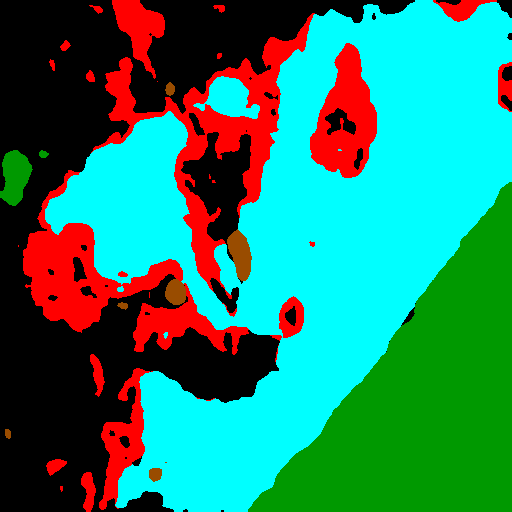
\includegraphics[width=0.22\textwidth]{figures/patch_img_seg_test/1/111_4_2019-04-30_S1_GRD_VVVH_patch_42_mask_rgb_aspp.png}
    &
    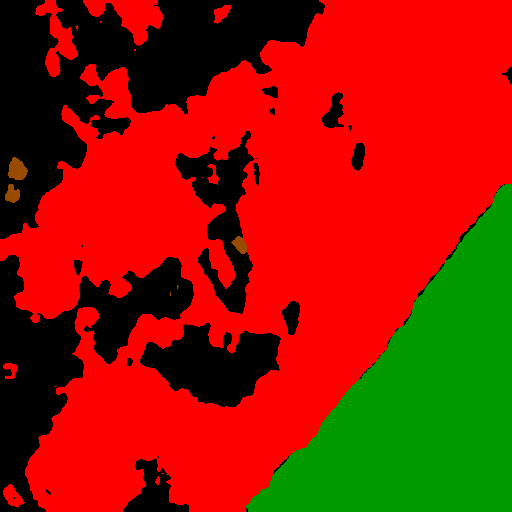
\includegraphics[width=0.22\textwidth]{figures/patch_img_seg_test/1/111_4_2019-04-30_S1_GRD_VVVH_patch_42_mask_rgb_deeplab.png}
    &
    
    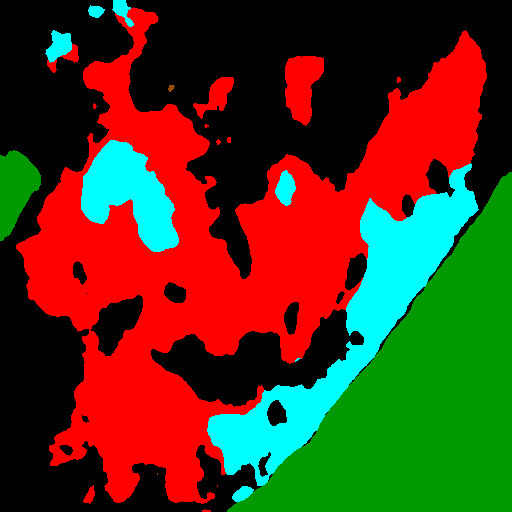
\includegraphics[width=0.22\textwidth]{figures/patch_img_seg_test/1/111_4_2019-04-30_S1_GRD_VVVH_patch_42_mask_rgb_unet.png}
    \\[0.5em]
    % Row 2: folder “2”
    \num\putindeepbox[b]
    \includegraphics[width=0.22\textwidth]{figures/patch_img_seg_test/2/129_2_2020-03-19_S1_GRD_VVVH_patch_70}
    &
    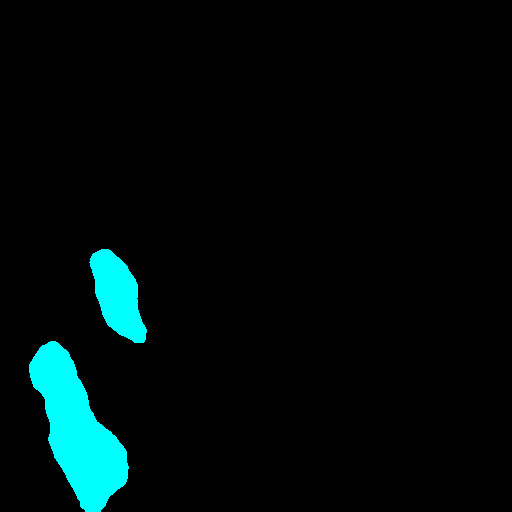
\includegraphics[width=0.22\textwidth]{figures/patch_img_seg_test/2/129_2_2020-03-19_S1_GRD_VVVH_patch_70_mask_rgb_aspp.png}
    &
    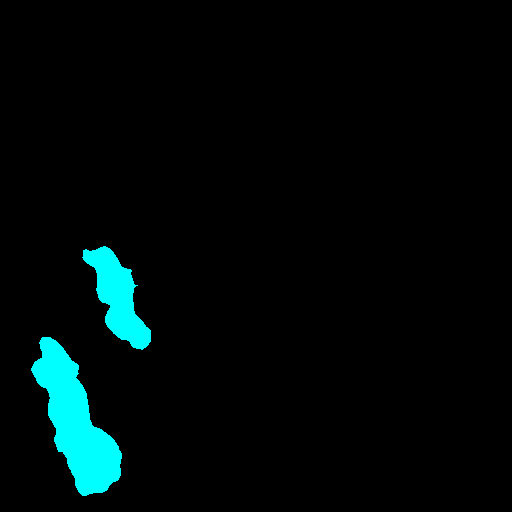
\includegraphics[width=0.22\textwidth]{figures/patch_img_seg_test/2/129_2_2020-03-19_S1_GRD_VVVH_patch_70_mask_rgb_deeplab.png}
    &
    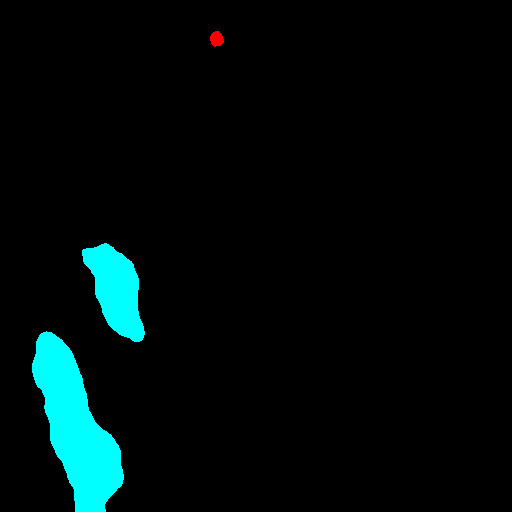
\includegraphics[width=0.22\textwidth]{figures/patch_img_seg_test/2/129_2_2020-03-19_S1_GRD_VVVH_patch_70_mask_rgb_unet.png}
    \\[0.5em]
    % Row 3: folder “3”
    \num\putindeepbox[c]
    \includegraphics[width=0.22\textwidth]{figures/patch_img_seg_test/3/146_1_2021-05-22_S1_GRD_VVVH_patch_18}
    &
    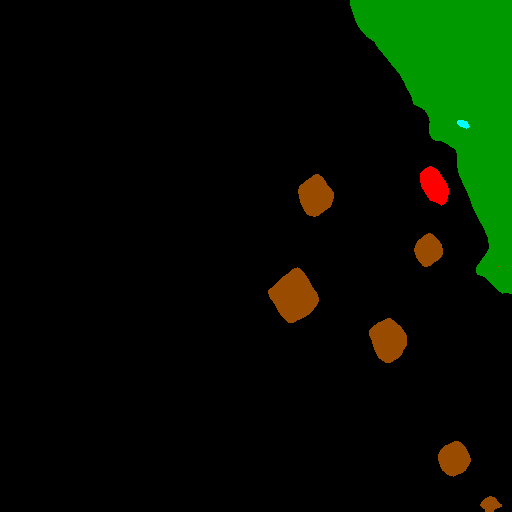
\includegraphics[width=0.22\textwidth]{figures/patch_img_seg_test/3/146_1_2021-05-22_S1_GRD_VVVH_patch_18_mask_rgb_aspp.png}
    &
    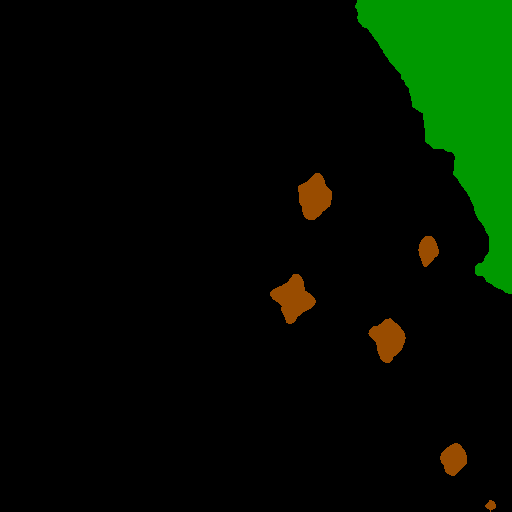
\includegraphics[width=0.22\textwidth]{figures/patch_img_seg_test/3/146_1_2021-05-22_S1_GRD_VVVH_patch_18_mask_rgb_deeplab.png}
    &
    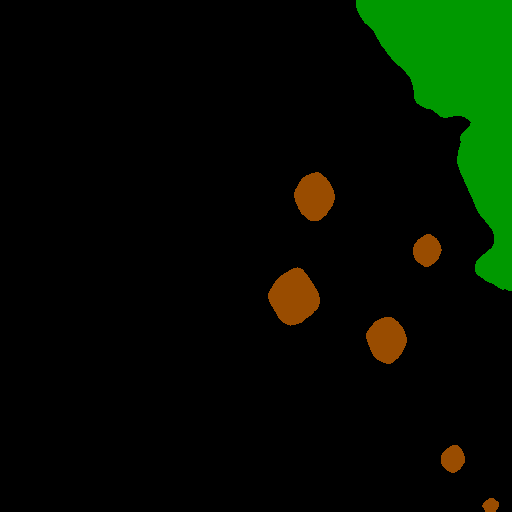
\includegraphics[width=0.22\textwidth]{figures/patch_img_seg_test/3/146_1_2021-05-22_S1_GRD_VVVH_patch_18_mask_rgb_unet.png}
    \\[0.5em]
    % Row 4: folder “4”
    \num\putindeepbox[7pt]
    \includegraphics[width=0.22\textwidth]{figures/patch_img_seg_test/4/148_1_2021-11-18_S1_GRD_VVVH_patch_30}
    &
    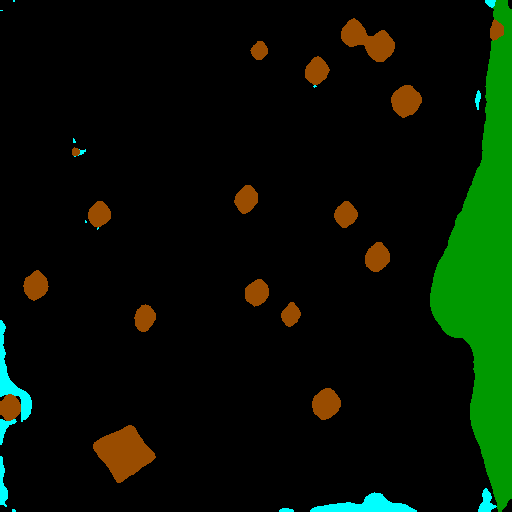
\includegraphics[width=0.22\textwidth]{figures/patch_img_seg_test/4/148_1_2021-11-18_S1_GRD_VVVH_patch_30_mask_rgb_aspp.png}
    &
    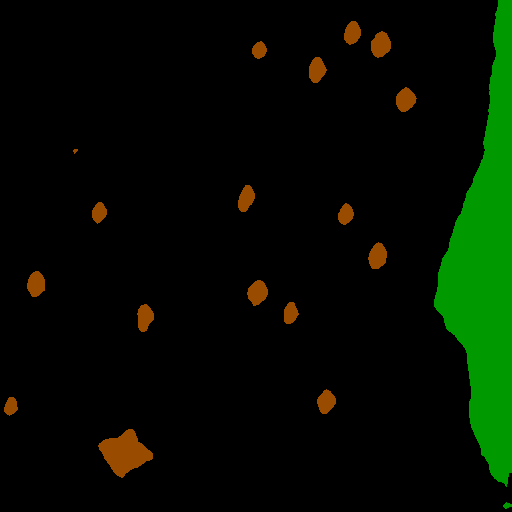
\includegraphics[width=0.22\textwidth]{figures/patch_img_seg_test/4/148_1_2021-11-18_S1_GRD_VVVH_patch_30_mask_rgb_deeplab.png}
    &
    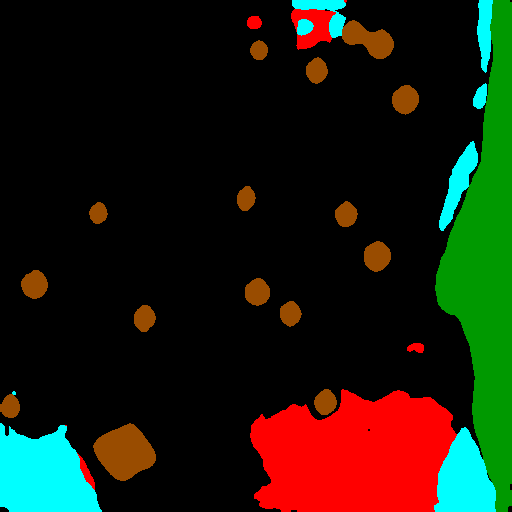
\includegraphics[width=0.22\textwidth]{figures/patch_img_seg_test/4/148_1_2021-11-18_S1_GRD_VVVH_patch_30_mask_rgb_unet.png}
    \\
  \end{tabular}
  \caption{Patch‐level segmentation comparison across four Peruvian scenes (folders 1–4). Columns are: (a) SAR images (b) Resnet_34_UNet_ASPP; (c) Resnet_34_DeepLabV3+; (d) Resnet_UNet_34.}
  \label{fig:patch_comparison}
\end{figure}



\paragraph{Per‐Scene Area Statistics}  
Table~\ref{tab:scene_areas_by_img} summarizes the distribution of oil and look‐alike coverage across eight Peruvian spill events that were part of the test split. This was generated via the Sentinel 1 images of size 5567x5567 at 10m resolution.  We observe a wide range of slick extents: the largest oil footprint occurs in scene \texttt{10016\_2} (31.6\,km\(^2\)), while the smallest appears in scene \texttt{146\_1} (0.39\,km\(^2\)). Look‐alike areas likewise vary from 6.16\,km\(^2\) (\texttt{10016\_2}) up to 18.34\,km\(^2\) (\texttt{111\_4}), reflecting either natural sea‐surface phenomena or residual spill artifacts. These per‐scene statistics highlight the severe class imbalance and the need for robust negative sampling: in scene \texttt{111\_4} the look‐alike area actually exceeds the true oil area, underscoring why our 1:1 sea‐only sampling was essential to teach the model local background variability.


\paragraph{Qualitative Segmentation Examples}  
Figure~\ref{fig:full_seg_examples} presents full‐image segmentation for four representative Peruvian spill scenes using the same model as the results in Table~\ref{tab:scene_areas_by_img}. In image (a), the model accurately delineates a narrow oil band along the coast, with only sparse false positives offshore. Image (b) demonstrates robustness to complex shoreline geometry: despite a jagged coast, the predicted mask tightly follows the true slick edge. The small spill in image (c)  tests sensitivity to sub-kilometer features; here the network successfully captures thin slick patches while largely ignoring surrounding look‐alikes. Finally, image (d) illustrates a challenging mixed case: most of the oil is correctly segmented, and look‐alike noise is largely suppressed, although a few isolated false positives remain near the shore. Together, these examples validate that our ResNet-34 UNet backbone fine-tuned on local data, can recover both large and fine-scale spills in operational SAR imagery.


\begin{table}[htbp]
\centering
\caption{Per-scene oil and look‐alike pixel counts and areas, indexed by image ID from Table~\ref{tab:peruvian_selection}.}
\label{tab:scene_areas_by_img}
\resizebox{\textwidth}{!}{%
\begin{tabular}{lrrrrr}
\toprule
\textbf{Img} & \textbf{Oil pixels} & \textbf{Oil area (km\(^2\))} & \textbf{Look‐alike pixels} & \textbf{Look‐alike area (km\(^2\))} \\
\midrule
14 & 316\,190 & 31.619 &  61\,659 &  6.1659 \\  % 2018-11-29
17 & 178\,057 & 17.8057 & 183\,415 & 18.3415 \\ % 2019-04-30
18 &  53\,028 &  5.3028 &  74\,673 &  7.4673 \\ % 2019-09-09
19 & 200\,777 & 20.0777 & 129\,578 & 12.9578 \\ % 2019-10-27
21 & 114\,574 & 11.4574 & 148\,100 & 14.8100 \\ % 2020-03-19
25 &   3\,938 &  0.3938 &  45\,980 &  4.5980 \\ % 2021-05-22
26 & 128\,597 & 12.8597 & 119\,963 & 11.9963 \\ % 2021-05-25
28 & 171\,286 & 17.1286 &  71\,314 &  7.1314 \\ % 2021-11-18
\bottomrule
\end{tabular}
}
\end{table}


\begin{figure}[htbp]
  \centering
  \begin{tabular}{cc}
    % Row 1
    \num\putindeepbox[a]{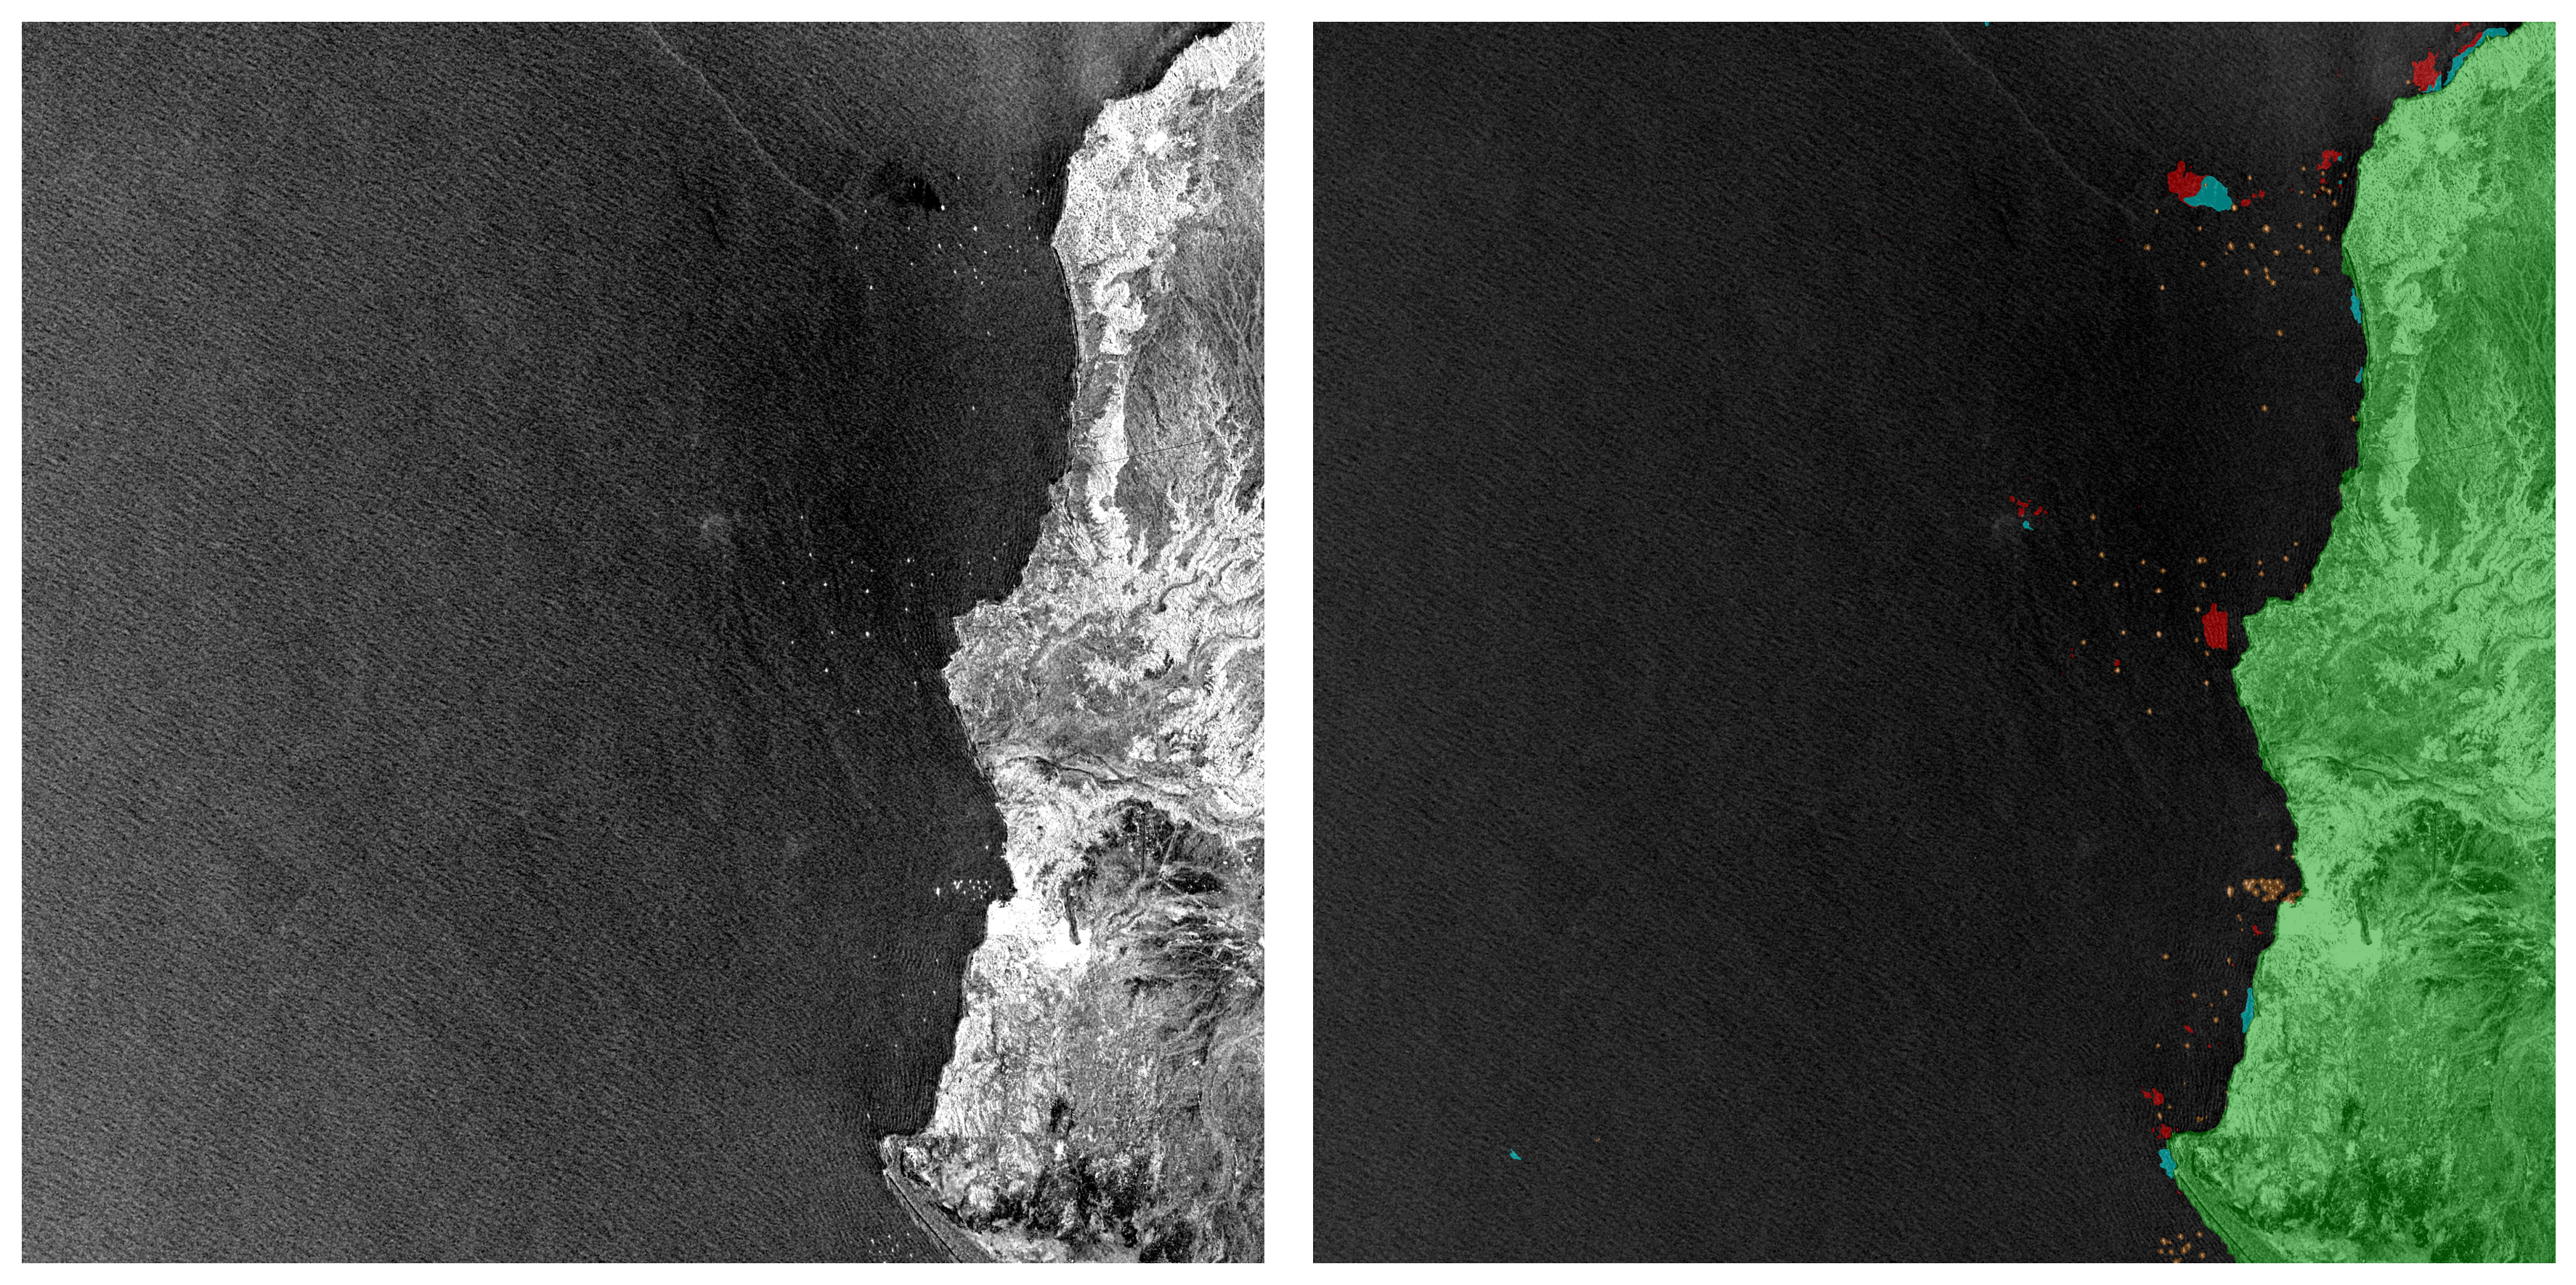
\includegraphics[width=0.45\textwidth]{figures/full_img_seg_test/118_1_2019-09-09.png}}
    &
    \num\putindeepbox[b]{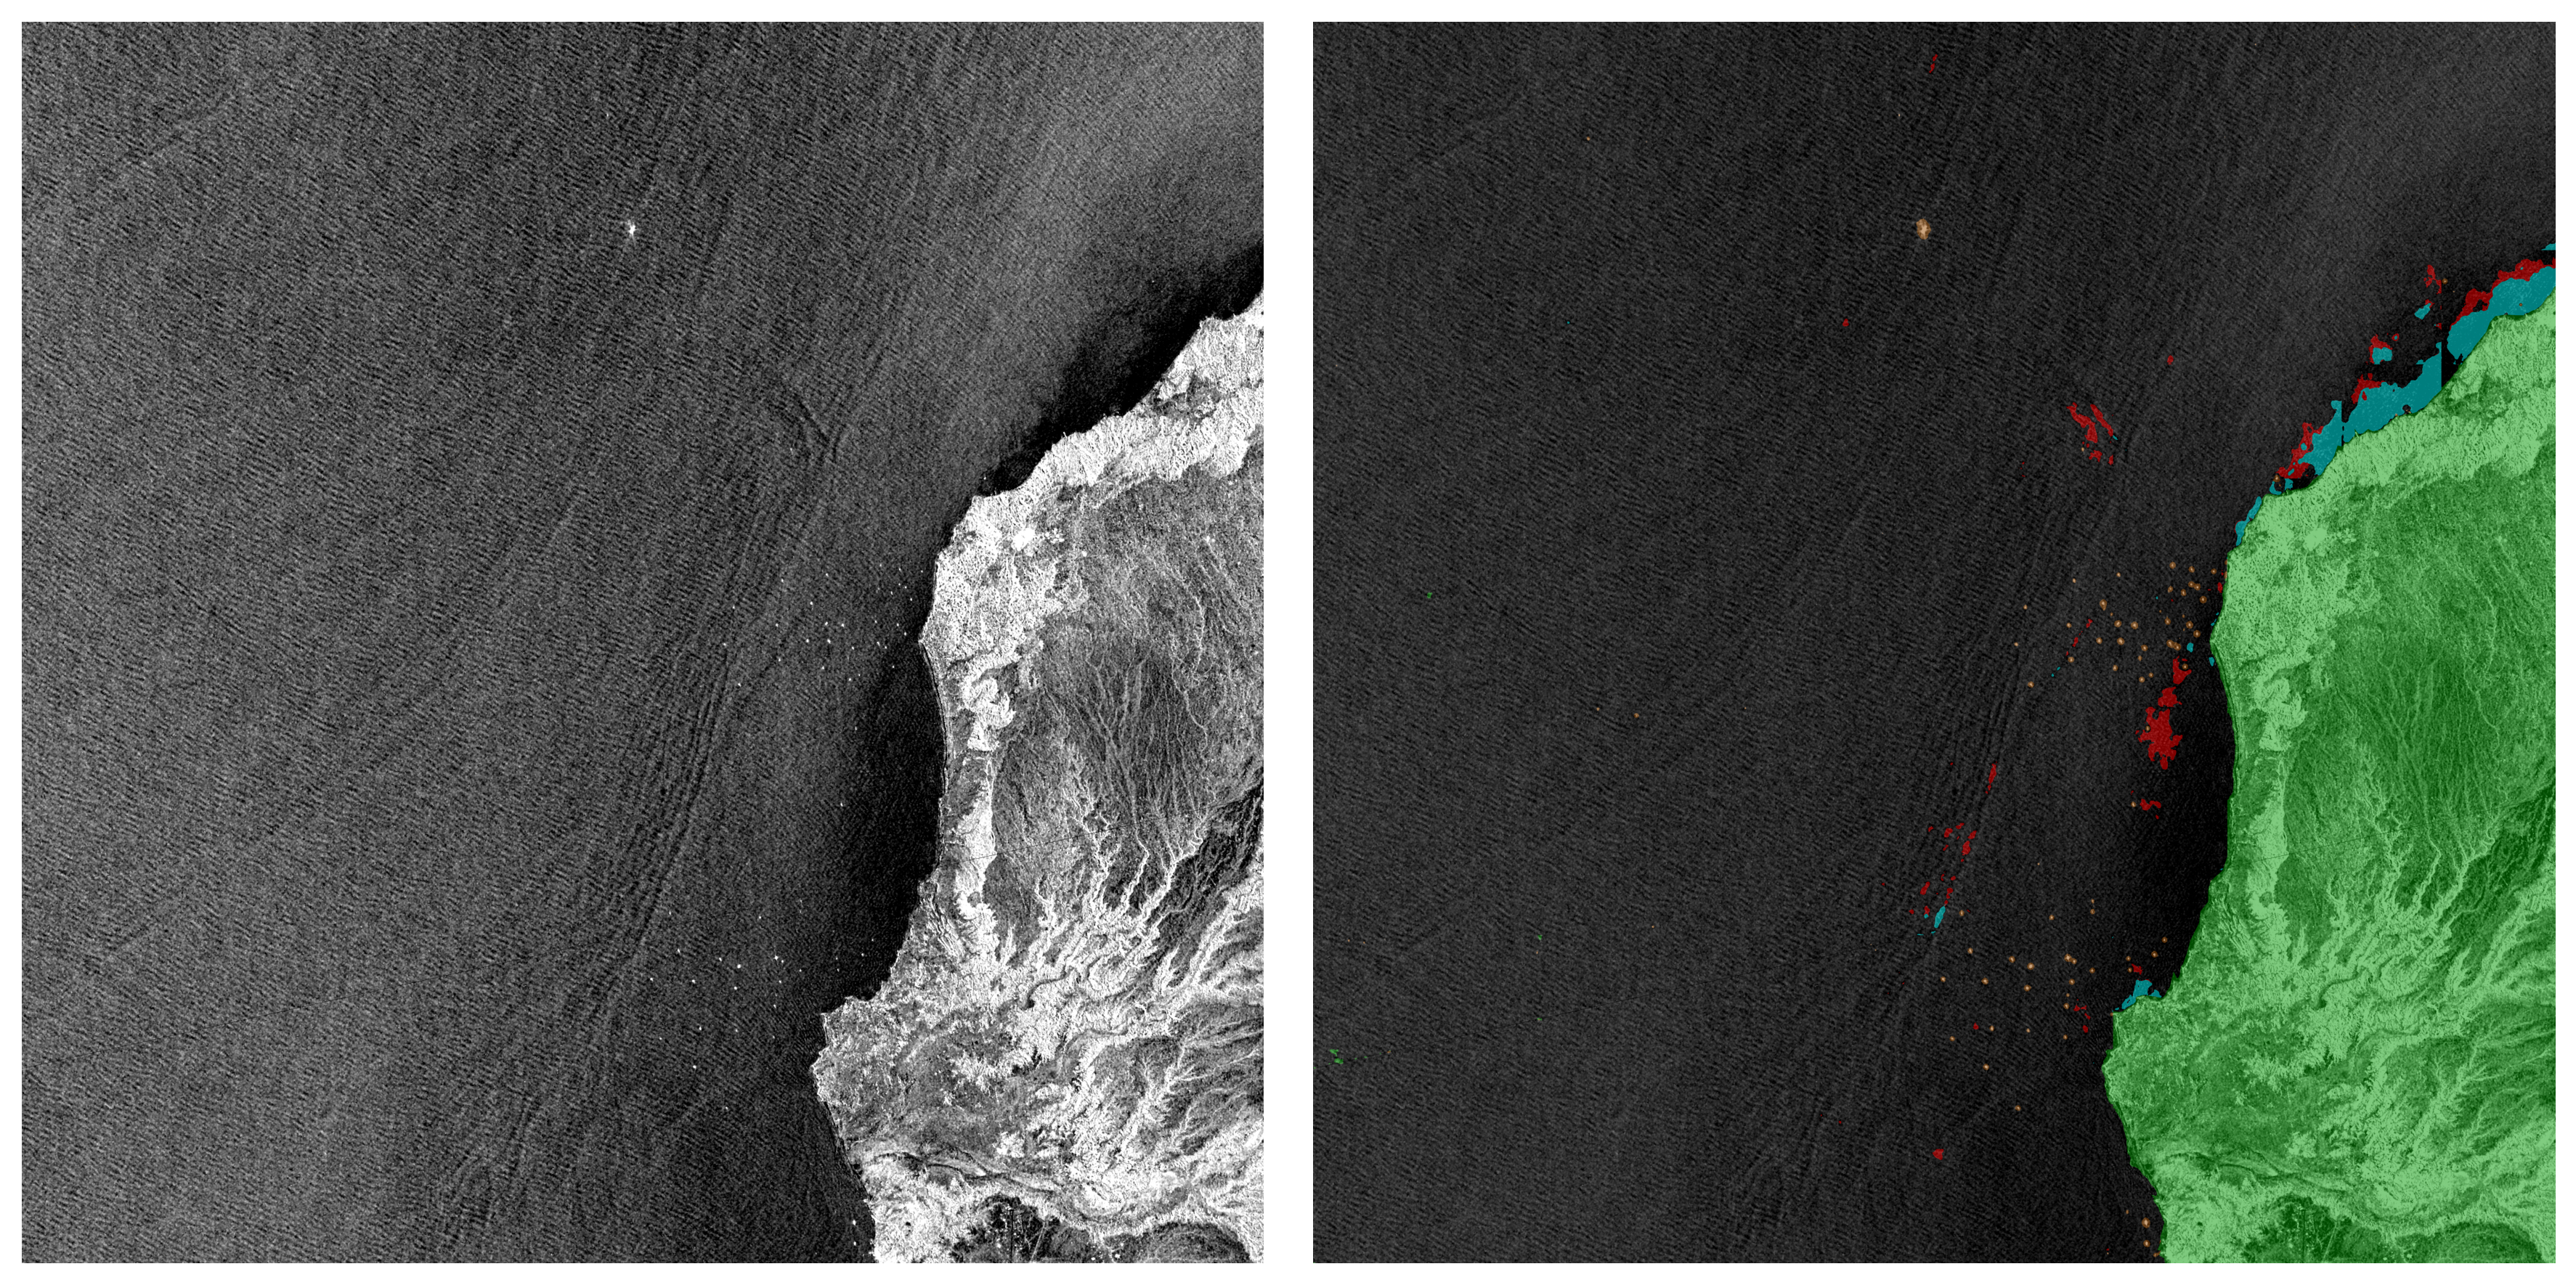
\includegraphics[width=0.45\textwidth]{figures/full_img_seg_test/120_4_2019-10-27.png}}
    \\[1em]
    % Row 2
    \num\putindeepbox[c]{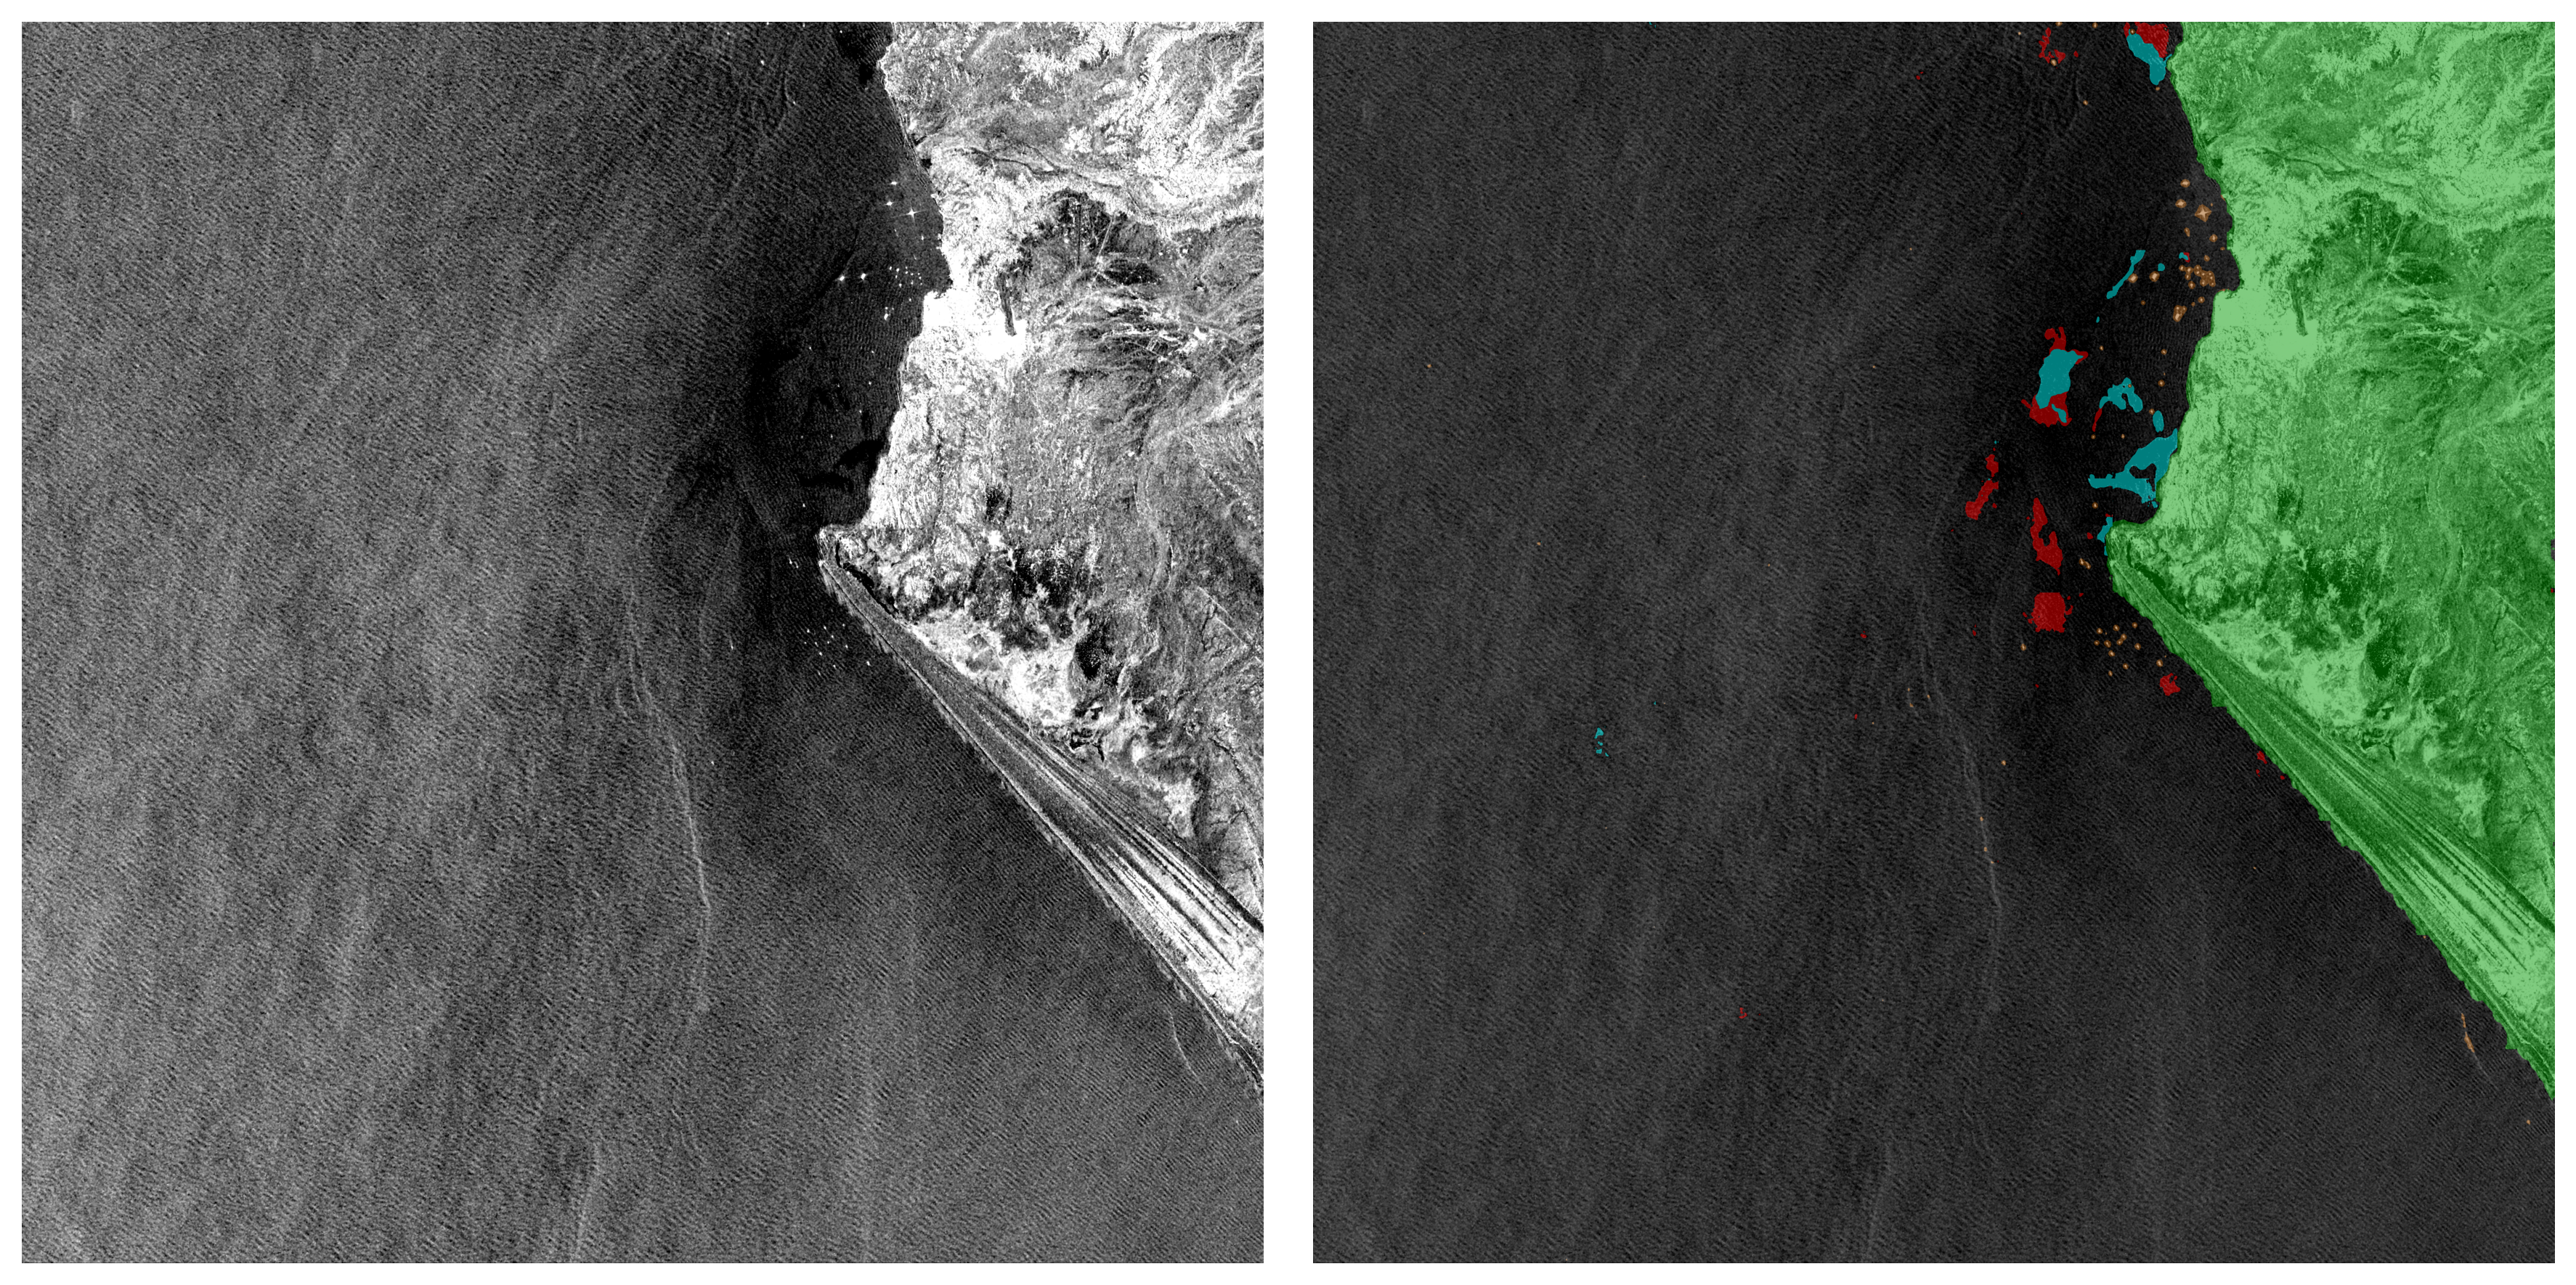
\includegraphics[width=0.45\textwidth]{figures/full_img_seg_test/146_2_2021-05-25.png}}
    &
    \num\putindeepbox[d]{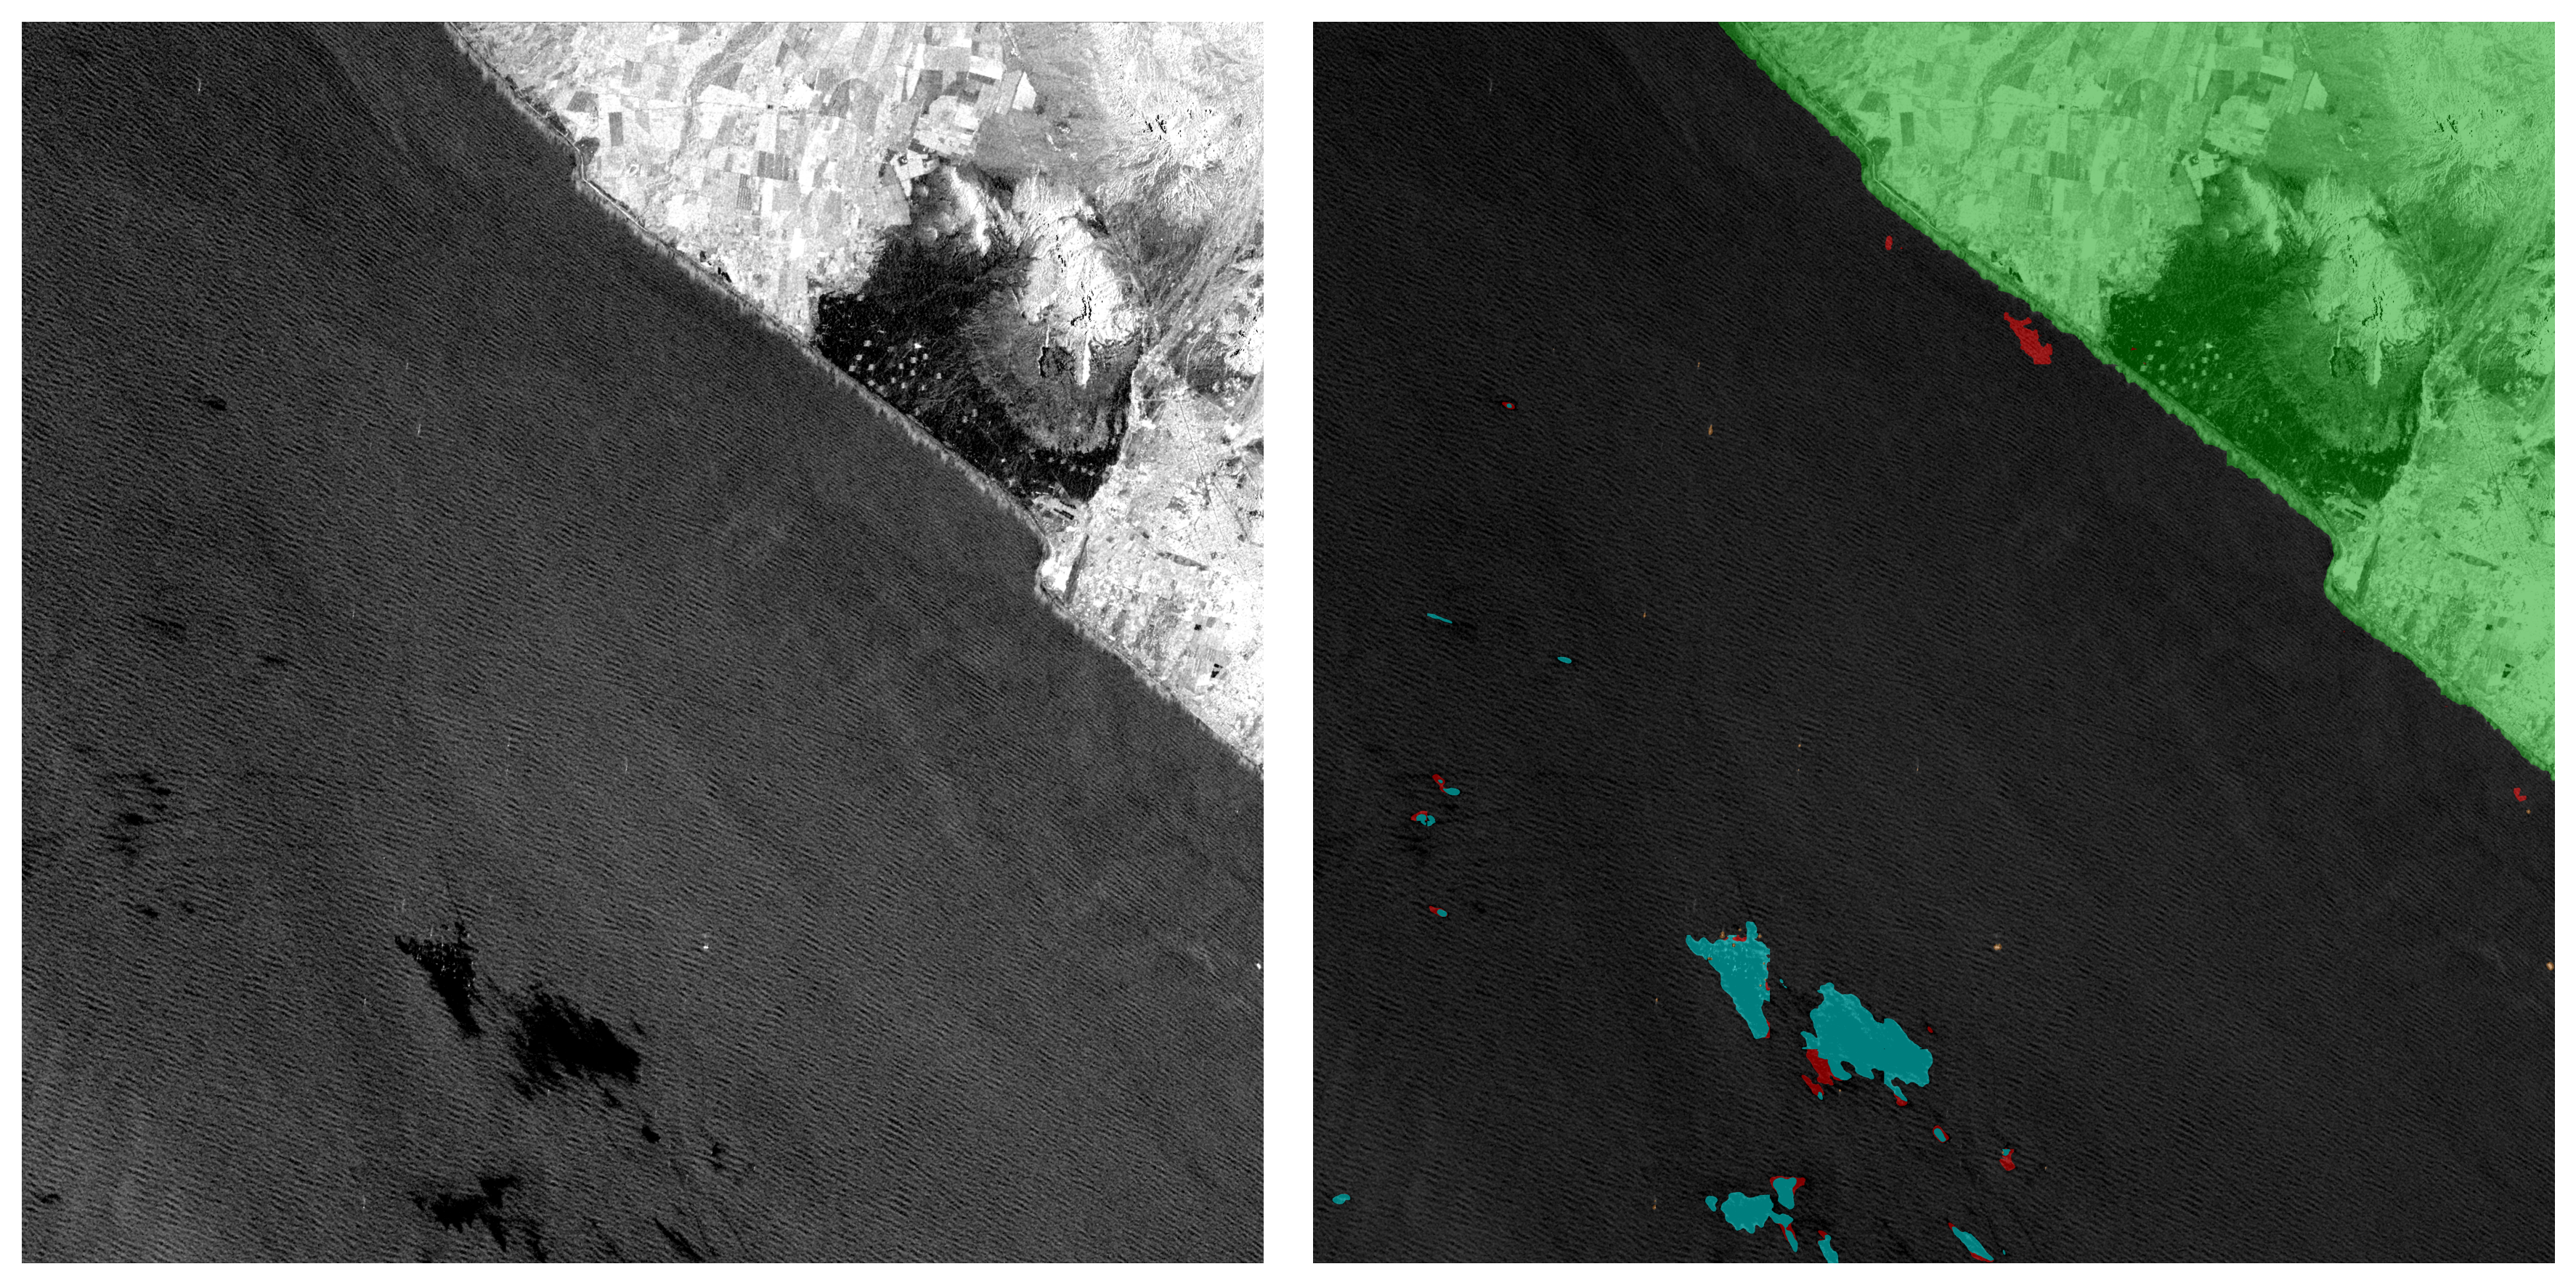
\includegraphics[width=0.45\textwidth]{figures/full_img_seg_test/10016_2_2018_11_29.png}}
    \\
  \end{tabular}
  \caption{Full‐image segmentation examples on four Peruvian spill scenes, referenced by image ID: (a) Img 18, (b) Img 19, (c) Img 26, (d) Img 14 (see Table~\ref{tab:peruvian_selection} for reference).}
  \label{fig:full_seg_examples}
\end{figure}






\clearpage


\section{Conclusions}

We have demonstrated that transferring deep segmentation models from a well-studied Mediterranean SAR dataset to the Peruvian coast requires explicit domain adaptation:

\begin{itemize}[leftmargin=*,label=\textbullet]
  \item \textbf{Source-only generalization fails:} Models trained solely on European waters drop from 67.8 \% mIoU to as low as 35.7 \% on Peruvian SAR scenes.
  \item \textbf{Fine-tuning is effective:} Supervising on just 2 132 local patches yields an average +12 pp gain in mIoU (40.1 \% → 51.9 \%), closing much of the domain gap.
  \item \textbf{Model trade-offs:}  
    \begin{itemize}
      \item UNet+ASPP attains the highest oil-spill IoU (13.2 \%),  
      \item DeepLabV3\texttt{+} excels on look-alikes (28.2 \%) and ship classes (34.5 \%),  
      \item Pure skip-based UNet maintains the lowest false-positive rates (< 1.1 \%), vital for operational reliability (See \ref{tab:resnet34_unet_fpr}
    \end{itemize}
  \item \textbf{Operational implications:} Multi-scale context modules boost recall but incur more false positives; skip-fusion architectures offer a precision–recall balance suited to real-world monitoring.
  \item \textbf{Future directions:} We plan to explore unsupervised domain adaptation methods, augment the training pool with synthetic cGAN-generated samples, and integrate models into near-real-time, on-board SAR processing pipelines.
\end{itemize}
\clearpage

\section{Appendix}



\begin{table}[p]
\centering
\caption{Sentinel-1 SAR images used in this study, ordered by spill date. Includes acquisition delay and patch counts for training and testing subsets.}
\label{tab:peruvian_selection}
\scriptsize
\begin{tabular}{|c|c|c|c|c|c|c|c|}
\hline
\textbf{Img} & \textbf{Spill Date} & \textbf{Latitude} & \textbf{Longitude} & \textbf{Acquisition Date} & \textbf{Δ Days} & \textbf{Patches} & \textbf{Split} \\
\hline
1 & 22/09/2014 & -80.7519 & -3.5860 & 11/10/2014 & 19 & 38 & Train \\
2 & 14/03/2015 & -81.2819 & -4.5736 & 16/03/2015 & 2 & 64 & Train \\
3 & 05/01/2016 & -71.3392 & -17.6346 & 13/01/2016 & 8 & 52 & Train \\
4 & 11/03/2016 & -79.0288 & -8.1117 & 26/03/2016 & 15 & 88 & Train \\
5 & 19/05/2016 & -81.2745 & -4.5963 & 30/05/2016 & 11 & 18 & Train \\
6 & 08/08/2016 & -71.3393 & -17.6346 & 22/08/2016 & 14 & 157 & Train \\
7 & 27/03/2017 & -81.2922 & -4.4562 & 13/04/2017 & 17 & 68 & Train \\
8 & 27/03/2017 & -81.2922 & -4.4562 & 01/04/2017 & 5 & 56 & Train \\
9 & 27/03/2017 & -81.2922 & -4.4562 & 16/04/2017 & 20 & 44 & Train \\
10 & 11/07/2017 & -81.2717 & -4.3194 & 18/07/2017 & 7 & 6 & Train \\
11 & 11/07/2017 & -81.2717 & -4.3194 & 21/07/2017 & 10 & 32 & Train \\
12 & 05/06/2018 & -77.1448 & -12.0472 & 17/06/2018 & 12 & 157 & Train \\
13 & 11/10/2018 & -77.1457 & -12.0472 & 27/10/2018 & 16 & 70 & Train \\
14 & 19/11/2018 & -79.0288 & -8.1117 & 29/11/2018 & 10 & 58 & Test \\
15 & 07/04/2019 & -81.3123 & -4.6213 & 18/04/2019 & 11 & 10 & Train \\
16 & 18/04/2019 & -81.2604 & -4.2810 & 18/04/2019 & 0 & 24 & Train \\
17 & 18/04/2019 & -81.2604 & -4.2810 & 30/04/2019 & 12 & 60 & Test \\
18 & 04/09/2019 & -81.3656 & -4.4692 & 09/09/2019 & 5 & 22 & Test \\
19 & 14/10/2019 & -81.2777 & -4.3096 & 27/10/2019 & 13 & 32 & Test \\
20 & 18/03/2020 & -81.2349 & -4.2436 & 31/03/2020 & 13 & 74 & Train \\
21 & 18/03/2020 & -81.2349 & -4.2436 & 19/03/2020 & 1 & 22 & Test \\
22 & 17/08/2020 & -81.3086 & -4.6100 & 22/08/2020 & 5 & 32 & Train \\
23 & 09/01/2021 & -81.3235 & -4.7120 & 25/01/2021 & 16 & 38 & Train \\
24 & 28/04/2021 & -81.2725 & -4.2896 & 10/05/2021 & 12 & 26 & Train \\
25 & 17/05/2021 & -81.3299 & -4.7144 & 22/05/2021 & 5 & 62 & Test \\
26 & 17/05/2021 & -81.3299 & -4.7144 & 25/05/2021 & 8 & 26 & Test \\
27 & 02/11/2021 & -81.3048 & -4.2936 & 18/11/2021 & 16 & 18 & Train \\
28 & 04/11/2021 & -81.2940 & -4.4414 & 18/11/2021 & 14 & 30 & Test \\
29 & 15/01/2022 & -77.1520 & -11.9256 & 02/02/2022 & 18 & 76 & Train \\
30 & 15/01/2022 & -77.1520 & -11.9256 & 25/01/2022 & 10 & 158 & Train \\
31 & 15/01/2022 & -77.1680 & -11.9638 & 25/01/2022 & 10 & 160 & Train \\
32 & 24/08/2022 & -81.2725 & -4.2896 & 30/08/2022 & 6 & 14 & Train \\
33 & 09/10/2022 & -81.0984 & -4.5111 & 17/10/2022 & 8 & 66 & Train \\
34 & 18/08/2023 & -81.2921 & -4.3025 & 25/08/2023 & 7 & 54 & Train \\
35 & 18/08/2023 & -81.2921 & -4.3025 & 03/09/2023 & 16 & 30 & Train \\
36 & 18/08/2023 & -81.2921 & -4.3025 & 22/08/2023 & 4 & 38 & Train \\
37 & 21/12/2024 & -81.3319 & -4.5322 & 07/01/2025 & 17 & 58 & Train \\
38 & 21/12/2024 & -81.3319 & -4.5322 & 29/12/2024 & 8 & 40 & Train \\
39 & 21/12/2024 & -81.3319 & -4.5322 & 26/12/2024 & 5 & 20 & Train \\
40 & 21/12/2024 & -81.3319 & -4.5322 & 10/01/2025 & 20 & 34 & Train \\
\hline
\end{tabular}
\end{table}

% Table for ResNet-34 UNet
\begin{table}[htbp]
\centering
\caption{Per‐scene performance and false‐positive rates for ResNet-34 UNet on the Peruvian test set.}
\label{tab:resnet34_unet_fpr}
\small
\begin{tabular}{lcccc}
\toprule
\textbf{Scene} & \textbf{mIoU} & \(\mathrm{FPR}_{\mathrm{total}}\) & \(\mathrm{FPR}_{\mathrm{oil}}\) & \(\mathrm{FPR}_{\mathrm{look}}\) \\
\midrule
14 & 67.41\% & 0.58\% & 0.23\% & 0.15\% \\
17 & 61.93\% & 0.59\% & 0.15\% & 0.19\% \\
18 & 44.71\% & 1.51\% & 0.16\% & 0.29\% \\
19 & 59.80\% & 0.54\% & 0.10\% & 0.21\% \\
21 & 60.32\% & 1.42\% & 0.30\% & 0.60\% \\
25 & 53.89\% & 0.89\% & 0.01\% & 0.18\% \\
26 & 59.25\% & 1.50\% & 0.27\% & 0.38\% \\
28 & 54.70\% & 0.85\% & 0.51\% & 0.17\% \\
\bottomrule
\end{tabular}
\end{table}

% Table for ResNet-34 UNet+ASPP
\begin{table}[htbp]
\centering
\caption{Per‐scene performance and false‐positive rates for ResNet-34 UNet+ASPP on the Peruvian test set.}
\label{tab:resnet34_unet_aspp_fpr}
\small
\begin{tabular}{lcccc}
\toprule
\textbf{Scene} & \textbf{mIoU} & \(\mathrm{FPR}_{\mathrm{total}}\) & \(\mathrm{FPR}_{\mathrm{oil}}\) & \(\mathrm{FPR}_{\mathrm{look}}\) \\
\midrule
14 & 66.43\% & 1.00\% & 0.34\% & 0.49\% \\
17 & 59.55\% & 1.21\% & 0.23\% & 0.73\% \\
18 & 42.42\% & 1.60\% & 0.25\% & 0.41\% \\
19 & 58.96\% & 1.01\% & 0.12\% & 0.68\% \\
21 & 58.19\% & 3.10\% & 0.32\% & 2.31\% \\
25 & 53.04\% & 0.93\% & 0.03\% & 0.23\% \\
26 & 56.42\% & 1.56\% & 0.42\% & 0.46\% \\
28 & 53.19\% & 0.74\% & 0.48\% & 0.10\% \\
\bottomrule
\end{tabular}
\end{table}

% Table for ResNet-34 DeepLabV3+
\begin{table}[htbp]
\centering
\caption{Per‐scene performance and false‐positive rates for ResNet-34 DeepLabV3\texttt{+} on the Peruvian test set.}
\label{tab:resnet34_deeplabv3_fpr}
\small
\begin{tabular}{lcccc}
\toprule
\textbf{Scene} & \textbf{mIoU} & \(\mathrm{FPR}_{\mathrm{total}}\) & \(\mathrm{FPR}_{\mathrm{oil}}\) & \(\mathrm{FPR}_{\mathrm{look}}\) \\
\midrule
14 & 67.11\% & 0.55\% & 0.42\% & 0.00\% \\
17 & 63.48\% & 0.57\% & 0.15\% & 0.23\% \\
18 & 46.18\% & 1.18\% & 0.10\% & 0.33\% \\
19 & 62.14\% & 1.84\% & 0.15\% & 1.55\% \\
21 & 59.54\% & 4.92\% & 0.36\% & 4.28\% \\
25 & 54.99\% & 0.50\% & 0.01\% & 0.02\% \\
26 & 59.69\% & 1.31\% & 0.24\% & 0.47\% \\
28 & 54.15\% & 0.37\% & 0.23\% & 0.00\% \\
\bottomrule
\end{tabular}
\end{table}




\clearpage
\printbibliography
\end{document}
